% -------------------------------------- Directives for arara --------------------------------------

% arara: lualatex: { shell : yes }
% arara: biber
% arara: lualatex: { shell : yes }
% arara: lualatex: { shell : yes }

% ----------------------------------------- Document class -----------------------------------------

% Options:
% - `thesis=B` - bachelor's thesis
% - `thesis=M` - master's thesis
% - `czech` - thesis in Czech language
% - `english` - thesis in English language
% - `hidelinks` - remove colour boxes around hyperlinks
\documentclass[thesis=M,english]{template/FITthesis}[2019/12/23]

% ------------------------------------------- Typography -------------------------------------------

\usepackage{luavlna}
\usepackage[all]{nowidow}
\usepackage{csquotes}

% ------------------------------------- Bibliography settings --------------------------------------

\usepackage[style=iso-numeric]{biblatex}
\addbibresource{bibliography.bib}

% --------------------------------------------- Lists ----------------------------------------------

\usepackage{enumitem} % Enables e.g. `\begin{enumerate}[label=\textbf{F\arabic*}, ref=\labelenumi]`

% --------------------------------------------- Links ----------------------------------------------

\usepackage{xurl}

% ------------------------------------------- Footnotes --------------------------------------------

% https://tex.stackexchange.com/questions/28465/multiple-footnotes-at-one-point#comment288652_28467
\let\oldFootnote\footnote
\newcommand\nextToken\relax
\renewcommand\footnote[1]{%
    \oldFootnote{#1}\futurelet\nextToken\isFootnote}
\newcommand\isFootnote{%
    \ifx\footnote\nextToken\textsuperscript{,}\fi}

% ----------------------------------------- Code listings ------------------------------------------

\usepackage{minted}
\counterwithin{listing}{chapter}

% ----------------------------------------- Directory tree -----------------------------------------

\usepackage{dirtree}

% -------------------------------------------- Metadata --------------------------------------------

\assignment{assignment}
\department{Department of Software Engineering}
\title{Decentralized and Open Architecture of a Reservation System}
\authorGN{David} % Author's given name/names
\authorFN{Straka} % Author's surname
\authorWithDegrees{Bc. David Straka} % Author's name with academic degrees
\author{David Straka} % Author's name without academic degrees
\supervisor{doc. Ing. Tomáš Vitvar, Ph.D.}
\acknowledgements{I would like to start by thanking my supervisor, doc. Ing. Tomáš Vitvar, Ph.D., for his guidance and support throughout my work on this thesis, as well as for the time he dedicated to the consultations needed especially during the formative stages of the process. Furthermore, I would like to thank my family and friends for their support. Last but not least, I want to express my gratitude to the authors of the many tools and libraries that were used during my work on the thesis, as well as to the open source community as a whole.
}
\abstractCS{\begin{sloppypar}
Tato práce se zabývá návrhem, implementací a otestováním otevřené a decentralizované architektury pro univerzální rezervační systém. V práci je zahrnut přehled vybraných existujících rezervačních systémů a analýza požadavků. Tato práce dále navrhuje vhodnou architekturu, klientskou rezervační aplikaci a její back end, který je navržen tak, aby podporoval společný rezervační protokol založený na HTTP. Nakonec je představena implementace návrhu spolu s výsledky jeho testování a evaluace.
\end{sloppypar}
}
\abstractEN{This thesis deals with the design, implementation, and testing of an open and decentralized architecture of a general-purpose reservation system. The thesis first features an overview of select existing reservation systems and a requirements analysis. It then designs a suitable architecture, booking client application, and its back end, which is designed to support a common HTTP-based booking protocol. Lastly, an implementation of the design is presented, along with the results of its testing and evaluation.
}
\placeForDeclarationOfAuthenticity{Prague} % Where you have signed the declaration
\keywordsCS{decentralizovaná architektura, rezervační systém, decentralizace, rezervace, schůzky, Web}
\keywordsEN{decentralized architecture, reservation system, decentralization, reservations, bookings, appointments, Web}
\declarationOfAuthenticityOption{5} % Select as appropriate, according to the desired license
\website{https://davidstraka.dev/masters-thesis} % Optional URL (remove entirely if you have no URL for this thesis)

% -------------------------------------- End of the preamble ---------------------------------------

\begin{document}

% ----------------------------------------- Vlna settings ------------------------------------------

\singlechars{czech}{AaIiVvOoUuSsZzKk} % Add non-breaking space after "a" (https://github.com/michal-h21/luavlna/issues/10)
\singlechars{english}{AaIiVvOoUuSsZzKk} % Add non-breaking space after "a" (https://github.com/michal-h21/luavlna/issues/10)
\enablesplithyphens{english}

% ------------------------------------------ Introduction ------------------------------------------

\begin{introduction}
	\label{part:introduction}
	The online reservation service Reservio~\cite{reservio} claims that 70\% of people prefer to book online, and providing online bookings leads to a 30\% profit increase for businesses. One of the reviews showcased on their website~\cite{reservio} from the University Hospital Brno cites that these services save the hospital over 10 hours a week of administrative work.

A 2019 United States healthcare report by KPMG~\cite{kpmg_healthcare_2030}, on the other hand, claims that \enquote{most consumers prefer to book appointments by phone,} but it also states that about 40\% are unable to do so on the first try and that 58\% of millennials and 64\% of people belonging to the generation X \enquote{value online booking to the extent that they would switch providers in order to do so.}

According to a 2014 study on the adoption, use, and impact of electronic booking in private medical practices in Canada~\cite{pare_medical_ebooking}, both patients and physicians showed growing interest in such system, \enquote{great majority of patients said that they appreciated the system mainly because of the benefits they derived from it, namely, scheduling flexibility, time savings, and automated reminders that prevented forgotten appointments,} and the study's findings \enquote{suggest that the system's automated reminders help significantly reduce the number of missed appointments.}

Yet, in practice, one can see many businesses still opting not to offer online bookings, instead relying mainly on phone calls or sometimes emails for reservations.

When businesses do offer online bookings, they tend to use a wide variety of different systems, each with its own user interface (UI) and user experience (UX). This can be confusing for the customers and can lead to a suboptimal UX due to, for instance, having to learn to use a new UI and familiarizing oneself with the features available within the system, having to manage many different user accounts' login credentials (oftentimes leading to password reuse and thus also posing a security risk), and keeping track of all the bookings spread across the different platforms. Smaller booking systems also tend to struggle with handling surges in traffic. Because of the lack of standardization, migrating from one system to another can prove to be a challenge for both the business and the customers, risking vendor lock-in.

An alternative to having many different booking systems could be one or a few of them becoming dominant within its market. This does have the advantages of a unified UX and fewer login credentials; however, there are many disadvantages and risks associated with such dominant platforms (often dominant to the point of them becoming monopolies or oligopolies). Such risks can be seen in many other types of online services, such as social media, search engines, and e-commerce platforms. Once these dominant platforms form, they can be very difficult for users to escape, for instance, due to the network effect where~\cite{investopedia_network_effect} \enquote{increased numbers of people improve the value of a good or service,} and which~\cite{investopedia_network_effect} also says may lead to less innovation.

% https://www.grammarly.com/blog/spelling-e-mail-email/
With the rise of these dominant platforms, there has also been a growing number of efforts to create decentralized alternatives. Such decentralized systems often provide many of the advantages of a dominant centralized platform, such as being able to interact with a large network of users from a single client application with a familiar UI/UX and a single user account, but without many of the risks associated with the system being run by a single legal entity. An example of such an emerging decentralized system is the Fediverse. Some great examples of older decentralized online systems that are nowadays ubiquitous are email, and even the World Wide Web itself.

The goal of this thesis is to explore the possibility of creating a decentralized, general-purpose online reservation system by designing an open architecture of such system, including a common HTTP-based client-server protocol, and developing a reference implementation including both a client application and a back end. The created solution should be easy to integrate with state-of-the-art cloud-native architectures and should support a use case for a selected type of reservation business. Possible extensions for the selected use case should be discussed. The reference implementation should be tested and evaluated for the selected use case. Additionally, the thesis will explore select existing online reservation systems.

\end{introduction}

% ---------------------------------- Existing Reservation Systems ----------------------------------

\chapter{Existing Reservation Systems}
\label{part:existing_reservation_systems}

This chapter serves as an overview of select existing online reservation systems and can be taken as a form of market research for the booking system to be created.

The overview is meant to be qualitative rather than quantitative, focusing on the exploration of features provided by a select few systems and the user experience while using those systems. The systems chosen for the overview are Acuity Scheduling\footnote{Acuity Scheduling (\url
{https://www.acuityscheduling.com})}, Reservio\footnote{Reservio (\url
{https://www.reservio.com})}, Square Appointments\footnote{Square Appointments (\url
{https://squareup.com/us/en/appointments})}, and Wix\footnote{Wix (\url
{https://www.wix.com})}.

The criteria used to choose the systems for the overview are the following:
\begin{itemize}
    \item \textbf{Popularity} --- The system must be popular with the public. Without an extensive quantitative survey, this is a difficult criterion to evaluate. As a rough estimate, the system's ranking in the Google search results for the queries \enquote{online reservation system,} \enquote{online booking system,} and \enquote{online scheduling system} was used. If the systems appeared on the first couple of pages of the results, they were considered popular enough. Some flaws of this approach are, for instance, results personalization based on geographic location, as well as search engine optimization (SEO) techniques used by the systems. Similarly, different systems could have been discovered by using other search queries and search engines. However, despite the flaws of this approach, it still seemed to yield good enough results.
    \item \textbf{Localization} --- The system must have English localization.
    \item \textbf{Price} --- The system must offer a free version of its service (at least as a limited-time trial). Additionally, it must not require payment information to sign up for the free version.
\end{itemize}

\section{Acuity Scheduling}
\label{part:acuity_scheduling}

Acuity Scheduling~\cite{acuity} describes itself as \enquote{an online appointment-booking tool} that \enquote{is great for any business that needs clients to book appointments for services in advance.} It also says that \enquote{businesses including yoga studios, massage therapists, acupuncture, life coaches, photographers, hair and nail salons use Acuity with great success,} but that it \enquote{is not a great fit for businesses that want to book appointments that last more than a day, like car rentals, vacation rentals, or hotels.} Acuity Scheduling is a subsidiary of Squarespace -- a company that primarily focuses on providing a website-building service (for some time after Squarespace acquired Acuity, the scheduling product was rebranded to Squarespace Scheduling, but that change has since been reverted).

The website offers a free limited-time trial, after which it cannot be used without paying for one of its tiered plans. After first singing up for a business account, the user is asked for the name of their business and the name of an Acuity Scheduling subdomain that the service will create for the booking website of the business (this is optional, and if not provided, the website will be available under a shared subdomain and a URL query parameter with a generated identifier).

The user then creates their first appointment type by filling out the name of the appointment, its duration, whether it is a one-on-one appointment or a group appointment, and optionally, its price. If the user has selected the group appointment type, they must set the number of open slots per class as well.

Moreover, the user sets up the availability of the created appointment type by selecting a date and a time, whether or not it is a recurring event, and, if it is, the frequency of the recurrence (such as every Monday, every other Tuesday, the first Wednesday of each month, or daily), and the number of recurrences.

Lastly, the user can optionally connect third-party payment processors (Stripe, Square, and PayPal) for collecting deposits or full payments for the appointment bookings. Long-term subscriptions are also supported. The service claims~\cite{acuity} that it does not take any commission on the payments and that the only fees are those charged by the payment processor.

After the business user completes the sign-up process, customers can access a booking website that is created for the business. Upon accessing the website, customers see the business information (with only the sign-up completed, that is just the business name), followed by a list of appointments to choose from, with each appointment featuring its name, time and date, duration, and a sign-up button. If the business user selected the group appointment type, there is also a quantity field above the appointment list and the number of free spots available under each appointment's sign-up button. Signing up for a selected appointment is followed by filling out personal information (a full name, an email address, and optionally a phone number). If there was no payment required, the customer completes the booking and receives an email with the details of their booking, a link to reschedule or cancel the appointment, and links to add the appointment to their calendar. The booking page can be seen in the figure~\ref{fig:acuity_scheduling}. The customer can use an account to manage their booked appointments, but it is purely optional, and they can still manage their bookings through the email links. There is also no way for the business to limit their appointments to only signed-in customers (the business can, however, ban clients by their email address).

The scheduling functionality can be integrated into any website built with Squarespace (which can then use a custom domain). There are also simple booking components that can be embedded into another website, in addition to the option to embed a booking page iframe. The booking website can be customized by choosing between a couple of predefined layouts and can also use custom CSS. The platform also features webhooks and an extensive application programming interface (API), which can be used to integrate it with other applications.

Business users can see all their appointments in a calendar overview, as well as all their clients. Under each appointment in the calendar, the user can see all signed-up customers, reschedule or cancel their bookings (when the business user does this, the affected customer can be notified by email, but there is also an option not to send this notification), and add private notes and tags for each customer. The user can manually add new attendees to each appointment (which can be useful, for example, when a customer wants to create a booking over the phone, but the business wants to have everything tracked in the booking system). There is also an option to send an email to all attendees of a selected appointment, in addition to SMS reminders. The business user can be notified of new activity by email as well, and they can synchronize their calendar with other popular calendar applications.

Appointment types can be further customized by adding a color and a picture. Users can make appointments private, in which case they are not visible to the public and can only be accessed through a direct link. There is an option to require clients to sign up for every recurrence of a recurring appointment and an option to disallow clients from booking multiple spots. Appointment types can also have a form added for the customers to fill out before booking an appointment. The form can consist of questions with answers of several different types, including a text field, a drop-down list, a checkbox, and even a file upload. The business information shown on the booking website can also be customized a bit further by, for instance, adding a logo, filling out rich content instructions for the customers, and changing to one of a few different languages.

Other features available include CSV import and export of clients and appointments, setting limits on how long before an appointment it can be canceled or rescheduled, and adding Google Analytics to the booking website. A business account may be used by multiple users with separate login credentials and role-based permissions.

\begin{figure}
    \centering
    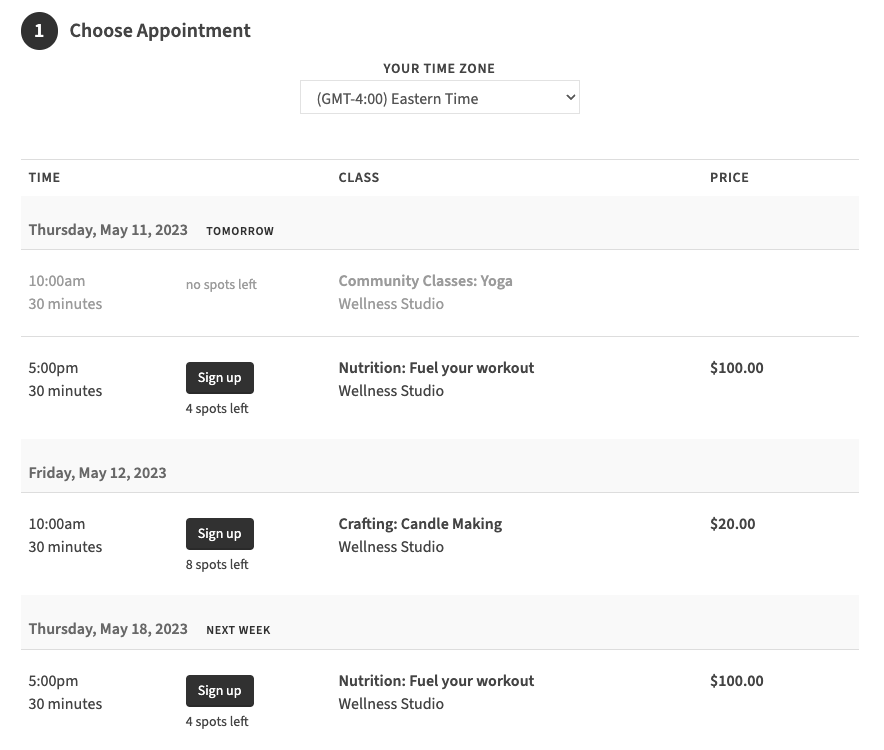
\includegraphics[width=1.0\textwidth]{content/existing_reservation_systems/acuity_scheduling.png}
    \caption[Acuity Scheduling]{Acuity Scheduling~\cite{acuity}}
    \label{fig:acuity_scheduling}
\end{figure}


\section{Reservio}
\label{part:reservio}

On the front page of its website~\cite{reservio}, Reservio describes itself as a \enquote{free online scheduling software for gyms, fitness centers, hair studios, barbershops, nail salons, car repair, medical services, teachers and educational institutions, group events, and more.}

When a user first signs up for a business account, they are asked to provide the following information:
\begin{itemize}
    \item the name of their business;
    % https://www.grammarly.com/blog/comma-between-correlative-conjunction-sets/
    \item the type of their business, which can be either \enquote{Single appointments} (described as \enquote{the client books a service or an appointment at a specific time}) or \enquote{Group events} (described as \enquote{host multiple clients at the same event, lecture or course}); to change this business type later on, one must contact customer support;
    \item opening hours, which \enquote{determine the exact range of when your clients can make bookings} and can also be customized per employee;
    \item the physical address of their business;
    \item optionally the contact phone number of their business;
    \item and optionally other information about their business -- a website, a slogan, a description, and additional information about the physical address.
\end{itemize}

Users are also asked to add the services they would like to provide to their clients. Each service must have a name and a duration, and can optionally have a description, a price, a color (to visually differentiate it from other provided services), and an additional question to ask the customers (which can also serve as an input for a voucher code).

Lastly, users can also add staff members of the business who provide the previously added services, each with a name, a checklist of the services they provide, and optionally a short biography.

After the user completes the sign-up process, customers can access a booking website that is created for the business on a Reservio subdomain. When a customer accesses the booking website, they immediately see all the information about the business that was provided during the sign up. They then select a service for booking, a staff member (or \enquote{anyone available}), a date from a calendar picker, and a free time slot for the selected date. The customer can complete their booking either as a guest or by creating a Reservio account (or logging into an existing account). If the customer chooses to create an account, they can also see their booking history and cancel their bookings (in the settings, a business can set how long before the event can the bookings be canceled). The business user can also restrict in the settings who can create bookings to for example only existing clients or only clients with an account. As the last step of the booking process, the customer can answer the additional question that was added by the business, and they may also add a note. Afterwards, the customer is sent an email with the details of their booking.

For group events, the process is very similar, with the business user additionally specifying the capacity of an event. The customers can then book multiple spots for an event, as long as there is sufficient space available. Group events can also be marked as private by the business user, in which case they are not visible to the public and can only be accessed through a direct link.

The booking page iframe or simple booking components can also be embedded into another website. The booking website can be set as indexable by search engines and can use a custom domain instead of the Reservio subdomain (for premium accounts only). The layout and theme of the booking website can be somewhat customized as well, though most of the customizations are limited to premium accounts. There is an extensive API which can be used to integrate Reservio with other applications.

Business users can see their existing bookings in a calendar (also available as per staff member and per service views) which can be seen in the figure~\ref{fig:reservio}, as well as an overview of their clients. Premium users can have their calendar be synchronized with other popular calendar applications. Users can edit and cancel the existing bookings, as well as manually add new bookings and clients. Unreliable clients can be blocked and there is a CSV file import of clients as well. The amount of bookings a business can have is limited by different premium subscription plans.

Other available features include the ability to receive email and SMS notifications about new and canceled bookings (though SMS is limited to premium accounts), client reminders a set number of days or hours before a booked event, the option to limit the time of user data retention, and adding analytics to the booking website (such as Google Analytics and Meta Pixel; limited to premium accounts). Businesses can opt in to have their profile listed in a service marketplace (which customers can access through a separate application). One business account may be used by more staff members with separate login credentials and role-based permissions.

The platform also features online payments (which can be set as mandatory or optional), for which it takes a commission: This feature includes the handling of refunds when a customer cancels their booking and the possibility of long term memberships. However, according to Reservio~\cite{reservio}, this feature is currently only available in the Czech Republic where the company originates and for security reasons it does not work when a custom domain is set up for the booking website.

\begin{figure}
    \centering
    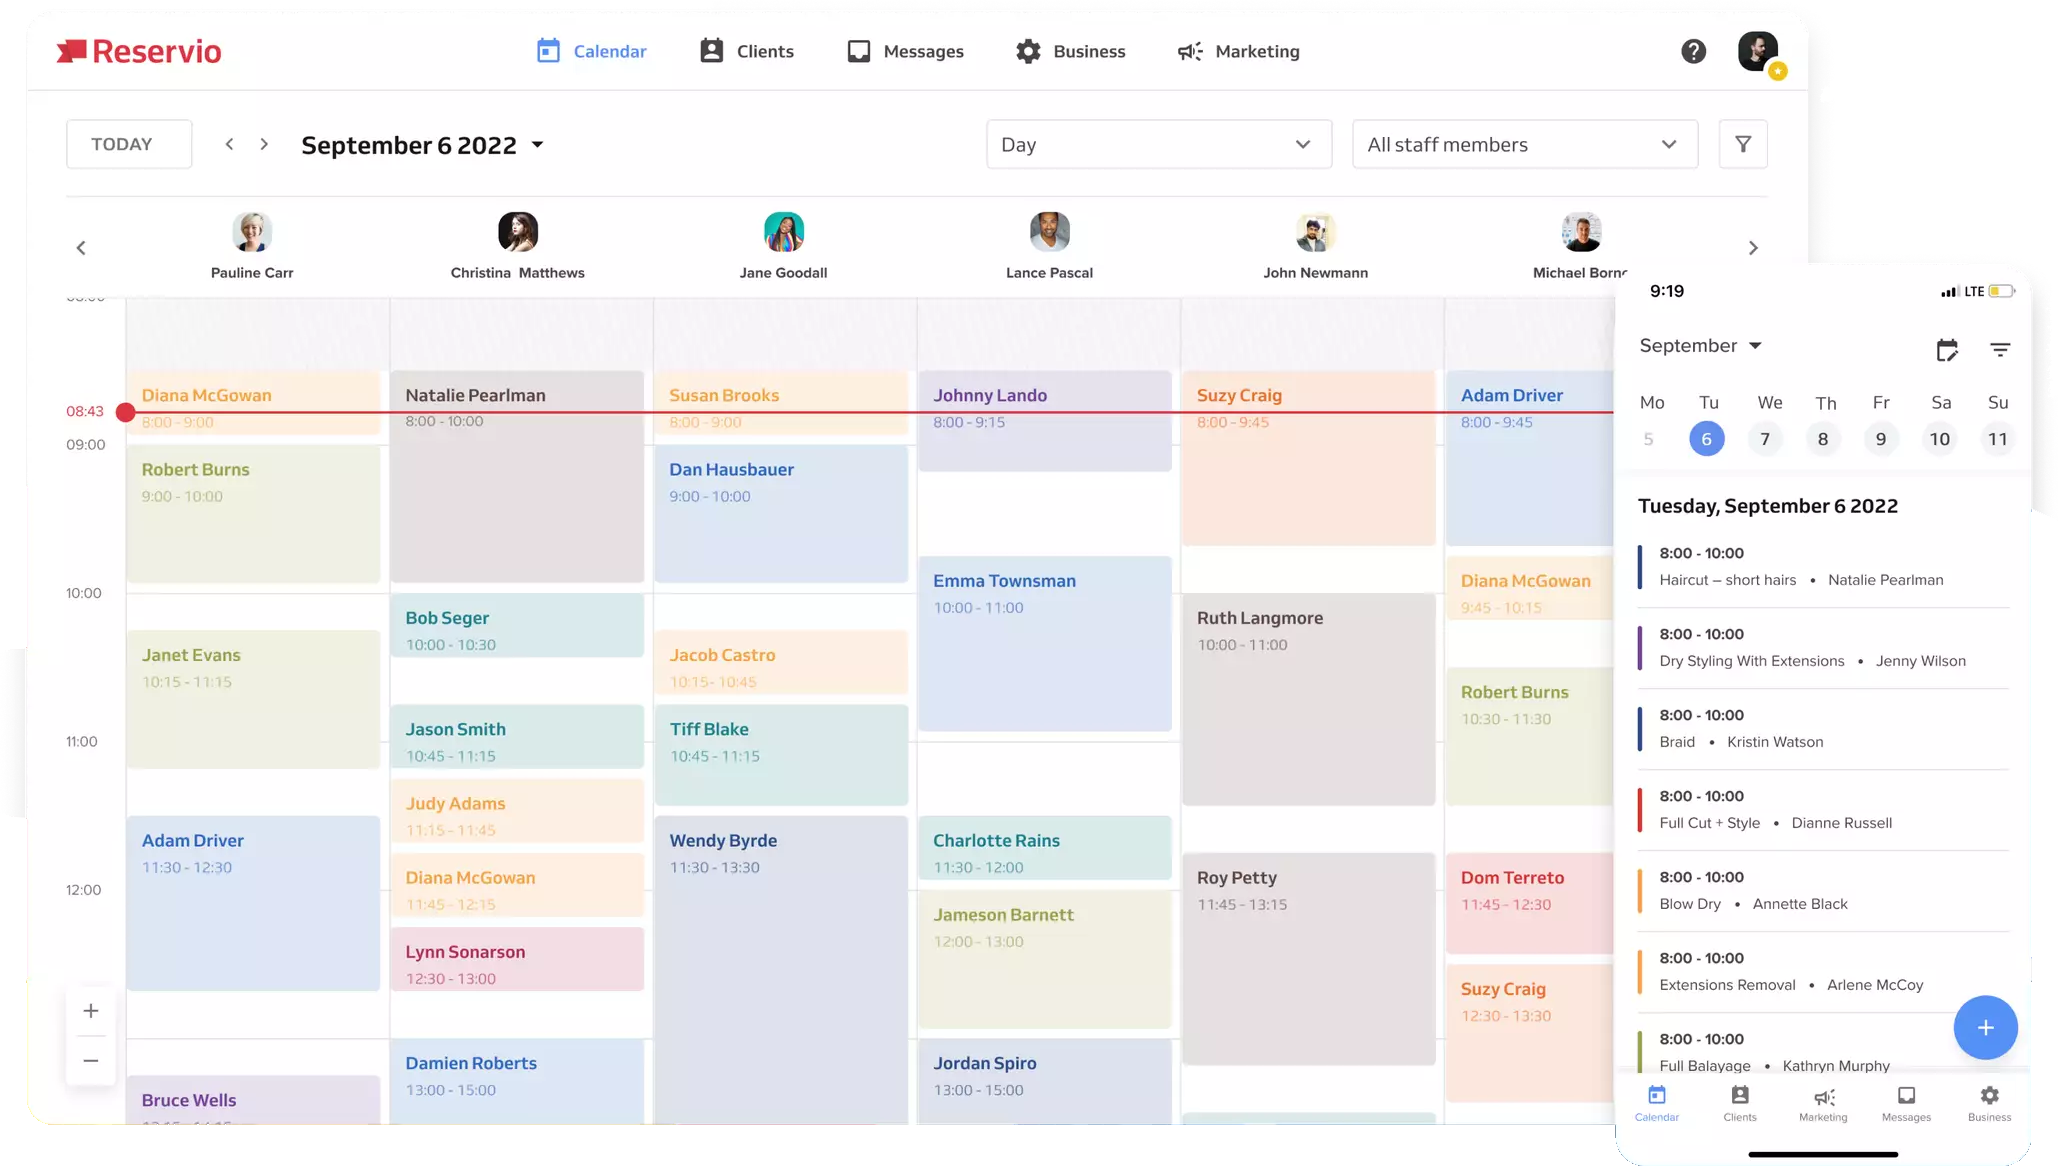
\includegraphics[width=1.0\textwidth]{content/existing_reservation_systems/reservio.png}
    \caption[Reservio]{Reservio~\cite{reservio}}
    \label{fig:reservio}
\end{figure}


\section{Square Appointments}
\label{part:square_appointments}

Square Appointments~\cite{square} is a product by the company Square (not to be confused with Squarespace, which is a different company), which primarily focuses on providing financial services to businesses (some other reservation systems mentioned in this overview even offer Square as a payment processor). Square Appointments~\cite{square} describes itself as \enquote{the all-in-one point of sale for
booking, payments, and more.}

After first signing up for a business account, the service asks the user to provide some basic information: their personal name, business name, business phone number, time zone, and the type of the business. This information is later shown to the customers on an online booking site, if the business chooses to have one.

Square also asks for the number of staff members, business locations, and optionally services offered. The user also must fill out their estimated monthly revenue and optionally can input the average price per client. Then the user selects which features they are interested in, which can be any of the following: customizable online booking site, selling products, accepting payments, prepayment and no-show protection, and automated reminders and confirmations. For the purposes of this overview, the customizable online booking site, as well as the automated reminders/confirmations were chosen.

Square Appointments offers a feature-limited free plan (which is also limited to a single business location), as well as a limited-time trial of their lowest tier paid plan. The trial was used for this evaluation.

In the administrative dashboard, the user can edit their business location details, including its physical address, contact information, and social media links. They can add a short description of their business, a logo, and business hours.

The user then creates services that they offer, by filling out the service name, description, price, and duration. The service can have an image attached to it and its business location specified (when the business has multiple locations). A cancellation fee can be set up, and there can be extra time added to be blocked off after the service is done (for example for cleaning). The service can be categorized and team members can be assigned to it.

Finally, the user enables online bookings and can set up a customizable Square Online website with booking functionality built in. This website is published to a Square provided subdomain, and a custom domain can be set up as well (with a premium account). The booking functionality can also be embedded into an existing website using a button component or an iframe.

When a customer visits the booking website, they can see basic information about the business (such as its name and phone number), the services they provide, their staff, and locations including the opening hours. To create a booking, the customer selects the services they want to book, the date from a calendar picker, one of the available time slots from a list, then they fill out their personal information (phone number, email address, and full name) and optionally any note for the business. If the business sets up multiple staff members for a service, the customer may select a preferred staff member as well.

Upon booking, Square automatically creates an account for the customer, which they can sign in using the provided phone number (this cannot be skipped). The booking can be added to their personal calendar by one of several popular calendar services. The customer can reschedule or cancel their booking. The customer also receives an email with the booking details.

The business user can view their calendar, which includes the customers' bookings. They can view each booking's details, edit and cancel the booking. Bookings can be added manually as well. The business calendar can be synchronized with Google Calendar. The business calendar can be seen in the figure~\ref{fig:square_appointments}.

In the settings, the business user can also choose to require manually accepting all bookings. Time limits for scheduling can be set as well. The list of staff can be removed from the booking website. An interesting feature is the so-called \enquote{Fake-it Filter} which lets the business \enquote{remove some of their availability to give the appearance that their business is busier.} Email and SMS reminders can be set up to be sent to the customers a given time before their appointment. There is no option to add a form to the booking process, but there is an option to create a form to send clients afterwards.

Other features include multiple team members using the business account with different permissions, a waiting list that automatically notifies clients of new availability, and an API. For some types of businesses, there is also a marketplace application from Square, where businesses can set up a profile for clients to discover. As square as a platform is primarily focused on offering financial services, there is a lot of detailed features related to this, including subscriptions management, thorough receipt customization, or various options regarding taxes, fees, and money transfers. Square also offers hardware for on location payments.

\begin{figure}
    \centering
    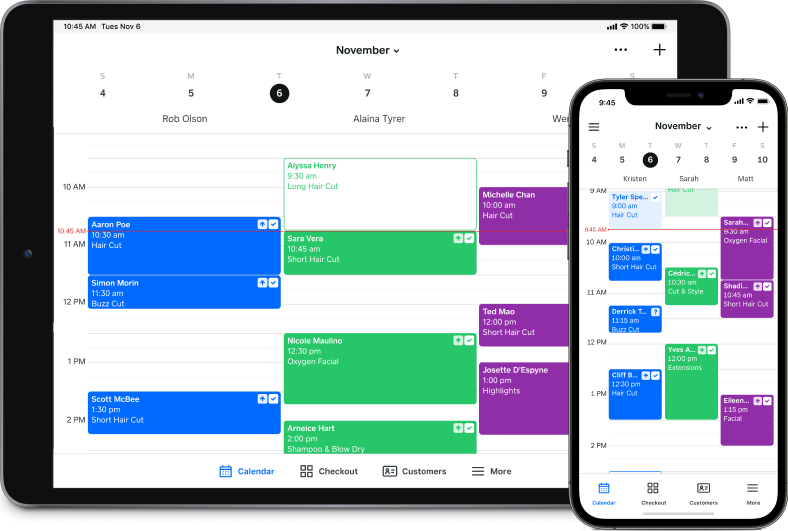
\includegraphics[width=1.0\textwidth]{content/existing_reservation_systems/square_appointments.png}
    \caption[Square Appointments]{Square Appointments~\cite{square}}
    \label{fig:square_appointments}
\end{figure}


\section{Wix}
\label{part:wix}

Wix~\cite{wix}, similarly to Squarespace (mentioned in a prior section of this overview), mainly offers a website building service which enables users to create their own websites using the Wix Website Builder UI. When building a website, users can make use of the so-called Wix Apps found in the Wix App Market. These can be thought of as plugins/extensions that the user can use to add functionality to their website or to the administrative dashboard. Wix Apps can be either official ones developed by Wix, or third-party ones (Wix provides an extensive API and even options to monetize the Apps published in the Wix App Market).

Wix offers three official Wix Apps which can in various ways be used to add reservation functionality to a Wix website: Wix Bookings, Wix Events, and Wix Restaurants. Wix Bookings seems to be meant for businesses offering frequently occurring appointments or classes. Wix Events appears more suited for those who organize events that only happen a few times or infrequently (Wix~\cite{wix} lists \enquote{planning a wedding, hosting a convention, or selling tickets to a show} as examples). Wix Restaurants, as the name suggests, focuses purely on restaurant businesses, enabling them to for example showcase their menu, receive orders, but also to set up online reservations.

This overview focuses on Wix Events, which are available as part of Wix's free plan (with some limitations), and briefly on Wix Bookings, which do not work with the website as part of the free plan, but do at least let users set up the administrative section.

After first signing up for an account, Wix asks the user a few questions about the purpose of their website to be built. Based on these answers it customizes the UI a bit, including adding suitable Wix Apps. When choosing the \enquote{Book Event} option as the primary focus of the website, the user is directed into the setup of the already installed Wix Events. They create their first event by entering the following:
\begin{itemize}
    \item the name of the event,
    \item the type of the event -- either a \enquote{Ticketed event} with options for pricing and availability or a \enquote{Registration only} event meant to collect confirmations of an invitation (RSVPs),
    \item the starting time and date of the event,
    \item optionally the ending time and date of the event,
    \item whether it is a recurring event (this lets the user add multiple dates/times for the event, but there does not appear to be an option to do this automatically),
    \item and optionally the location of the event (which can be a physical address or online).
\end{itemize}

The user can then add various tools to their website. These tools include for example a seating map which can \enquote{let guests choose their seats} or email marketing which can send invitations.

Lastly, the user can set up a custom domain to use for their website (though this is only available with a paid plan; otherwise the service provides a free Wix subdomain), design their website, and optionally optimize the website's SEO. If the user selected the \textit{Ticketed} event type, they also need to create ticket types for the created event to be bookable.

For designing the website, there are ready-made layouts which can be customized to a great extent, since that is Wix's primary focus. The user can also let the service use artificial intelligence (AI) to generate the website layout for them. Since this overview's goal is not to evaluate website builders, the AI option was chosen to save time. The resulting layout appeared fairly usable, though it seemed to have issues adjusting to different window sizes.

In the event details, the user can additionally provide a description and an image for the event. Events can be grouped into categories. Creating a ticket asks for the name of the ticket, optionally its description, the number of tickets available, a pricing method, and a window of time when the ticket is available for purchase. Tickets can be limited to a maximum amount per single order.

The pricing method can be fixed to a certain amount, split into different categories (e.g. child, adult), \enquote{pay what you want,} and free. Wix lets users connect third-party payment processors to collect these payments (such as PayPal and Stripe, but the availability of the payment processors depends on the user's country), and it charges a service fee (which is added on top of the payment processor's fee).

Events can have forms attached, which can include fields of multiple different data types. With the seating map tool, the user can create a detailed map of the seats and areas available at the event venue. They can then assign the available tickets to specific seats or areas. This seating map from the customer's perspective can be seen in the figure~\ref{fig:wix_seating_map}.

When all of this is set up, the user can publish the event on their website. Customers who access the website then navigate the event, see its details (such as the name, the time and date, and the location) and available tickets. If the window, during which tickets are up for sale, is open, they choose the ticket to buy by selecting the seat or admission area from the map (or, if no seating map was added, just choose which type of ticket to buy and its quantity), fill out any form the business user attached to the event, and check out. The customer can then download their tickets as a PDF document and add the event to their personal calendar. They also receive an email with the details of their booking.

The tickets that a customer receives include a QR code in them, which can then be scanned on location by the event organizer using a special-purpose mobile app from Wix. It does not appear that a customer can reschedule or cancel their booking, though the business user can do this for them (as well as cancel the event completely) through an overview of their orders and guests, though according to Wix~\cite{wix}, they will need to handle any refunds themselves. The business user can also add guests manually and later on manually check in any guest.

The Wix Bookings App adds a section with a booking calendar to the administrative dashboard. The user can add a service they would like to provide to their customers, which can be either an appointment (described as \enquote{a private session that can be booked according to availability}), a class (described as \enquote{a group session that can recur} where \enquote{clients book any session they want to join}), or a course (described as \enquote{a set of group sessions} where \enquote{clients book them all up front}).

In addition to providing some basic details about the service, the user can add pricing or a long-term membership plan, as well as staff members who provide the service. A booking form can also be attached. Unlike with Wix Events, the booking can be canceled or rescheduled by the customers, since there are options to disable this and limit the period of time before the booking when such changes can be made. Additionally, there is an option to require manually accepting all bookings.

The business user also sets up their opening hours, so that the service can offer recurring classes during these times (unlike with Wix Events, where recurring events had to have their times and dates added manually). A useful feature is also the option to schedule the appointment time slots either based on the service duration or every fixed amount of time. Booking reminders through email and SMS, calendar synchronization, and waiting lists are available as well. An example of a Wix website with the Wix Bookings functionality can be seen in the figure~\ref{fig:wix_bookings}.

Other features of the platform include built-in website analytics, multiple staff members managing a single account with role-based permissions, business website localization, CSV export of orders, and a full-featured API.

\begin{figure}
    \centering
    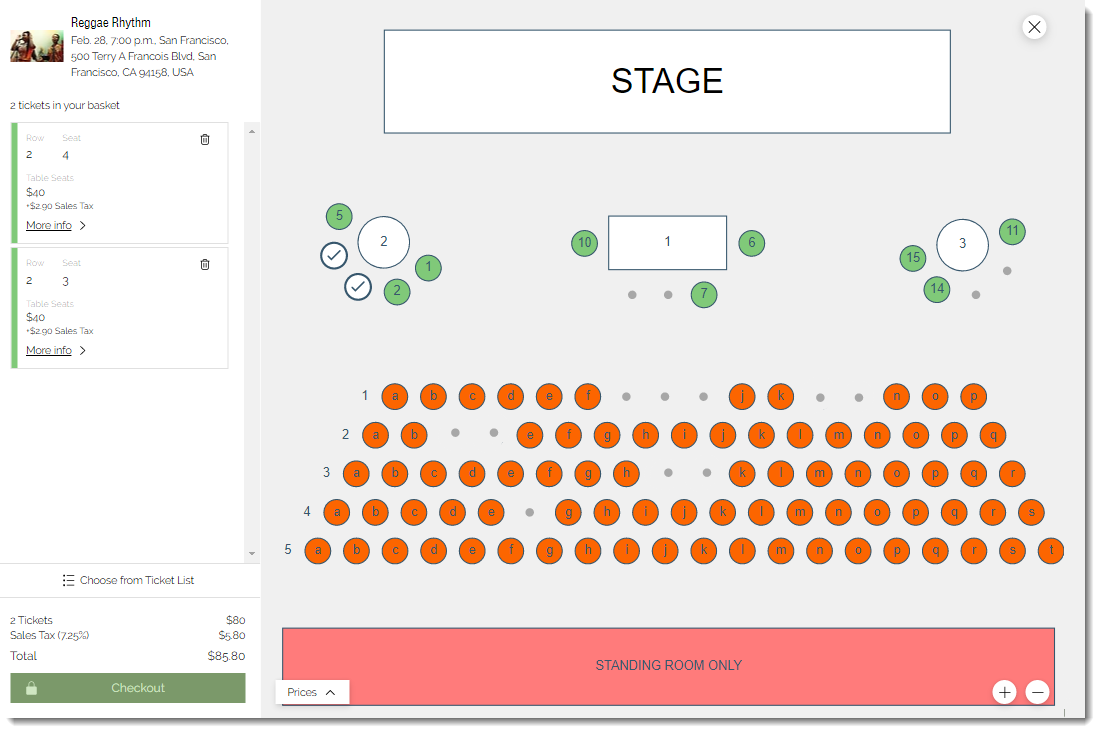
\includegraphics[width=1.0\textwidth]{content/existing_reservation_systems/wix_seating_map.png}
    \caption[Wix Events]{Wix Events~\cite{wix}}
    \label{fig:wix_seating_map}
\end{figure}

\begin{figure}
    \centering
    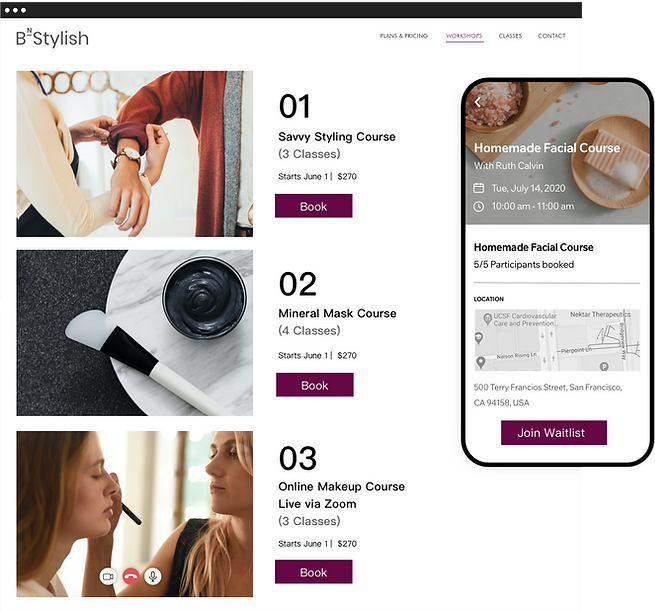
\includegraphics[width=1.0\textwidth]{content/existing_reservation_systems/wix_bookings.png}
    \caption[Wix Bookings]{Wix Bookings~\cite{wix}}
    \label{fig:wix_bookings}
\end{figure}


\section{Summary}
\label{part:existing_reservation_systems_summary}

To summarize this overview, among the four online reservation systems included in the overview -- Acuity Scheduling, Reservio, Square Appointments, and Wix -- there were many similarities and common features.

One of the similarities was the overall process of setting up a business account, filling out basic information about the business and setting up certain services, classes, or events for the clients to book. After this, the system would let the users create a booking website under the subdomain of the service or under a custom domain (which was always a premium feature). Customers could then access the website, view the information about the business, the services or events provided, and create a booking.

All systems also featured some options to accept payments, in addition to sending out emails with booking details and reminders. There was always some possibility to embed components or iframes with booking functionality to other websites, and an API for developers to integrate the system with other software (the API was always platform specific though). Calendar synchronization and multi-user accounts (with adjustable permissions) were also common features.

The main differences (excluding pricing strategies and the UI) seemed to be the ability to add forms for users to fill out during booking (present in Acuity Scheduling and in Wix's solutions), the ability to create a custom venue map with seating and areas sold under different ticket types (present in Wix Events).

Those platforms that focus on building websites (Wix and -- the owner of Acuity Scheduling -- Squarespace) offer more features for extensive booking website customization. On the other hand, Square Appointments from Square who focuses on financial services, offers the most features for payment processing, customer subscriptions, and financial reporting. Finally, Reservio seemed to offer subjectively the simplest business account setup and UI.



% -------------------------------------------- Analysis --------------------------------------------

\chapter{Analysis}
\label{part:analysis}

This chapter includes the analysis of functional and non-functional requirements for the system to be designed and implemented.

The requirements are based on both the assignment of the thesis, the overview of select existing reservation systems in the previous chapter~\ref{part:existing_reservation_systems}, and on original ideas for the new system.

\section{Functional Requirements}
\label{part:functional_requirements}

The functional requirements for the system are the following:
\begin{enumerate}[label=\textbf{F\arabic*}, ref=\labelenumi]
    \item \label{req:user_account} \textbf{User account} --- A user without an account must sign up for one to use the system. A user with a user account must be uniquely identified in the system. A user can log into their account and log out of their account.
    \item \label{req:inventory} \textbf{Inventory} --- A user can create an inventory of items for users to book. An inventory can have some basic information attached (such as a name, a description, and contact information). Items can also have information attached, and can be booked by multiple users up to a given maximum capacity.
    \item \label{req:booking} \textbf{Booking} --- A user can view an inventory including its items of a user with a created inventory. A user can book an item from an inventory. A user can view their existing bookings.
    \item \label{req:forms} \textbf{Forms} --- A user with an inventory can attach a form to the inventory. A user who wants to book an item from an inventory with a form must fill out the form.
    \item \label{req:deadlines} \textbf{Deadlines} --- A user with an inventory can limit until when an existing booking of an inventory item can be booked.
    \item \label{req:permissions} \textbf{Permissions} --- A user with an inventory can limit who can book items from their inventory by creating either an allowlist or a denylist of users.
    \renewcommand{\labelenumi}{\textbf{F\arabic{enumi}}*}
    \item \label{req:cancellation} \textbf{Booking cancellation} --- A user can cancel their existing booking. A user with an inventory can cancel an existing booking of item from their inventory as well.
    \item \label{req:edits} \textbf{Booking edits} --- A user can edit their existing bookings' form data.
    \item \label{req:ownership_verification} \textbf{Booking ownership verification} --- A user can easily verify in person that another user is the owner of a booking (for instance by scanning a QR code).
    \item \label{req:rt_updates} \textbf{Real-time item availability updates} --- A user can see real-time availability updates of a user with an inventory of items.
    \item \label{req:filtering} \textbf{Inventory filtering} --- A user can request a user's inventory of items filtered by item attributes.
    \item \label{req:custom_domain} \textbf{Custom domain} --- A user can use a custom domain for their identification in the system without setting up their own server.
    \item \label{req:data_exim} \textbf{Data export and import} --- A user can export and import their data in an open, standardized, machine-readable data format.
    \item \label{req:directory} \textbf{Inventory directory} --- A user with an inventory set up can opt in to have their inventory listed in a publicly accessible directory of user inventories. A user can access the directory of user inventories and filter/sort it by inventory attributes, or search it using natural language queries.
    \item \label{req:calendar_sync} \textbf{Calendar synchronization} --- A user can have their bookings with date and time attributes synchronized with their personal calendar. A user with an inventory set up can have their inventory items with date and time attributes synchronized with their business calendar.
    \item \label{req:notifications} \textbf{Notifications} --- A user can receive email (and possibly other types, such as SMS) notifications about their bookings and inventory items.
    \item \label{req:waitlist} \textbf{Waiting list} --- A user can enter a waiting list for an item that is fully booked. When a booking of that item is cancelled, or the user who the item's inventory belongs to increases the capacity, the item is automatically booked for the first users on the waiting list up to the newly available capacity.
    \item \label{req:payments} \textbf{Payments} --- A user with an inventory can require payments before or after a booking is made. A user can make a payment for a booking they made or are about to make, if that booking requires it.
    \item \label{req:multiuser_account} \textbf{Multi-user account} --- A user account can be used by multiple users. The user that first creates a user account can manage who else can use the account, and can limit their permissions.
    \item \label{req:internationalization} \textbf{Internationalization} --- A user can choose the locale (language, currencies, date and time formats, etc.) they want to use of the system under. A user with an inventory can set up their inventory with multiple different locales.
    \item \label{req:contacts} \textbf{Contacts} --- A user can add users with inventories to their contacts list. A user can view their contacts list and use it to quickly access the inventories of their contacts, as well as view the bookings made for the items of each individual contact.
    \item \label{req:autofill} \textbf{Autofill} --- A user can have their personal information automatically filled into forms during booking. This personal information can be manually entered by the user into a settings section, or automatically saved from previously filled-in forms.
    \item \label{req:automatic_reservations} \textbf{Automatic reservations} --- A user can instruct the system to automatically book selected items from selected inventories for them. Such instructions can for example be to book any appointment-type item at the beginning of every month from a given inventory, and that the event item must occur within a given time range.
\end{enumerate}

This list also includes some requirements that are out of scope for the initial version of the system, but are included for the sake of completeness. These requirements will not be further designed or implemented, but may have some impact for instance on the design of the system, the choice of technologies used, or certain implementation details. Such requirements are marked with an asterisk (\mintinline{text}{*}). Additionally, the item~\ref{req:permissions} will be only only designed, not implemented, to keep the scope of the project to a reasonable degree.

Most of the functional requirements stem from features already present some or all in the reservation systems previously explored. Optional requirement~\ref{req:automatic_reservations} is an original idea, that would could make use of the strengths of the newly designed system.


\section{Non-functional Requirements}
\label{part:non_functional_requirements}

The non-functional requirements for the system are the following:
\begin{enumerate}[label=\textbf{N\arabic*}, ref=\labelenumi]
    \item \label{req:decentralized_architecture} \textbf{Decentralized architecture} --- Users of the system can book from users regardless of the exact server or client application they use. Users can also set up their own server and client application to use the system.
    \item \label{req:cloud_native} \textbf{Cloud-native} --- The designed and implemented solution is containerized for easy deployment to a cloud platform and can be scaled well. The part of the solution that is responsible for the booking logic can be easily integrated into another solution.
    \item \label{req:general_purpose} \textbf{General-purpose} --- The designed and implemented solution should try to be as general-purpose as possible, not rigidly built around a very specific use case.
    \item \label{req:extensibility} \textbf{Extensibility} --- The designed and implemented solution can be extended both in terms of adding completely new functionality and extending existing functionality to better fit other use cases.
    \item \label{req:backward_compatibility} \textbf{Backward compatibility} --- Users of the system can book from users using servers that implement older or newer designs of the system (with the functionality limited to what both parties support).
    \item \label{req:fast_response_times} \textbf{Fast response times} --- As reservations in general can oftentimes be very time-sensitive, the system should be designed in such a way that does not introduce unnecessary delays to the booking process.
    \item \label{req:platform_agnostic} \textbf{Platform-agnostic} --- While testing the designed and implemented solution on a single platform should be sufficient for the purposes of this thesis (especially considering it is supposed to be a prototype and not a production-ready product), the solution should not be limited by its design or implementation to certain processor architecture, operating system, or a web browser (within reason, taking into account the commonplace platforms). An exception can be made for new standardized web technologies that are not supported by all platforms yet, as long as those technologies only add additional features.
    \item \label{req:open_source} \textbf{Open source} --- The designed and implemented solution is open-source, enabling anyone to freely use and repurpose it for their own needs.
\end{enumerate}

These requirements mostly originate from the assignment of this thesis, and in many cases present an improvement over existing reservation systems.



% --------------------------------------------- Design ---------------------------------------------

\chapter{Design}
\label{part:design}

This chapter describes the design of the proposed and implemented system. First it details the architecture, including the architecture of the decentralized booking system overall, the format of the booking addresses which are used to uniquely identify users within the system and the Uniform Resource Locator (URL) scheme which is to be used for distinguishing the booking addresses from other similar identifiers, and the architecture of the implementation in this thesis. Then the chapter describes the HTTP-based booking protocol which is used to communicate between different booking services. Lastly, the chapter describes the design of the individual back-end services and client application.

\section{Architecture}
\label{part:architecture}

% TODO reference requirements

This section first describes the architecture of the entire decentralized booking system, then later defines the format of booking addresses and their URI scheme, and lastly it focuses more on the architecture of the solution that is implemented in this thesis.

\subsection{System architecture}

Like many other decentralized systems, such as email, the Fediverse or Bluesky, the decentralized booking system shall use a federated architecture, which comprises of a network of several booking services operated by different booking service providers. These booking services shall communicate with each other using a common booking protocol, and interface with the end users through booking client applications provided by the booking service provider operating the booking service. Within the system, end users shall be uniquely identified by a booking address provided by their booking service provider. An end user can not only be a human, but also a bot, used to perform for instance automatic bookings, though some booking service providers and their users may opt to take measures to prevent bot traffic.

The common booking protocol shall be an application layer (as defined by~\cite{iso7498}) protocol built on top of the HTTP protocol (as per the thesis assignment). It shall be designed to be backwards-compatible, so that new features can be added without breaking compatibility with older versions of the protocol, and to be extensible, so that features useful to only some booking use cases can be added without affecting the rest of the protocol. The protocol's design is described in more detail in the section~\ref{part:booking_service}.

While the main intention is to design a system that is as interoperable as possible, some booking service providers may choose to ban traffic from other booking service providers if they act in malicious ways, and bookable users may choose to ban (or only allow) certain users as well. Booking service providers may even choose to completely isolate themselves from the rest of the system on the internet, and instead provide booking services on a private network only (this may be desirable for instance in some corporate environments).

A broad system network overview is shown in the figure~\ref{fig:system_network_diagram}. The figure~\ref{fig:system_conceptual_schema} then shows a detailed conceptual schema modelling the entities of the system and their relations.

The conceptual schema contains the following entities:
\begin{itemize}
    \item \textit{\textbf{BookingProtocol}} --- This entity represents the booking protocol used for communication between booking services in the system. It has the attribute \textit{version}, which is used to version the protocol in accordance with the principles of semantic versioning, described by~\cite{semver}. Such version shall, as~\cite{semver} says, be in the format \mintinline{text}{MAJOR.MINOR.PATCH}, where a \textit{MAJOR} version shall be incremented \enquote{when you make incompatible API changes,} a \textit{MINOR} version shall be incremented \enquote{when you add functionality in a backward compatible manner,} and a \textit{PATCH} version shall be incremented \enquote{when you make backwards compatible bug fixes.}
    \item \textit{\textbf{BookingProtocolExtension}} --- This entity represents any extension created for the booking protocol. It has the attributes \textit{id} and \textit{version}. The identifier \textit{id}, the entity's primary key, is used to uniquely identify the extension, and it shall be an Internationalized Resource Identifier (IRI), as defined by~\cite{rfc3987}. The \textit{version} is used to version the protocol extension, again in accordance with the principles of semantic versioning.
    \item \textit{\textbf{BookingService}} --- This entity represents a booking service, that is a server used to facilitate booking activities with other booking services in the system, using the booking protocol.
    \item \textit{\textbf{BookingServiceProvider}} --- This entity represents a provider of a booking service. Such provider is any individual or a company, that operates a booking service and issues booking addresses to its users.
    \item \textit{\textbf{BookingClientApp}} --- This entity represents a booking client application, that the end users use to interact with the booking service. Such application can be for instance a web application, a mobile application, or a desktop application with a graphical user interface (GUI), or even just a simple command-line interface (CLI).
    \item \textit{\textbf{User}} --- This entity represents an end user of the system. That can be both a human or a bot (or even a legal entity). One single person can also be represented as multiple users in the system, for instance if they use services of multiple booking service providers. This entity has the attribute \textit{bookingAddress} which is used to assign the user their system-wide unique booking address, and also serves as the entity's primary key. The format of the booking address is defined later on in this section.
    \item \textit{\textbf{BookableUser}} --- This entity extends the \textit{User} entity and it represents a user who has an inventory of items, that other users of the system can book.
    \item \textit{\textbf{Inventory}} --- This entity represents the inventory of a bookable user -- that is, again, a user who wants other users to be able to book items from them. The entity may have the attributes \textit{permissionMode}, \textit{metadata}, \textit{form}, \textit{itemType}, and \textit{itemMetadataSchema}.

    The attribute \textit{permissionMode} is used when the inventory features either a list of banned users who may not book items of the inventory or a list of allowed users who are the only ones permitted to book the inventory's items (which one of these options is used is determined based on the value of the attribute).

    The attribute \textit{metadata} is used to store arbitrary metadata about the inventory, such as contact information, opening hours, or announcements and notes for customers. To provide machine-readable semantic meaning to the metadata as well as the ability to link the data to other datasets, the JSON-LD format shall be used, as defined by~\cite{w3c_json_ld_1_0, w3c_json_ld_1_1}.

    The attribute \textit{form} is used to store a JSON Schema (as specified by~\cite{json_schema_spec}) which defines the structure of the data that the bookable user wants users to fill out when booking an item from the inventory. According to~\cite{json_schema}, the defined JSON Schema can then be used to both validate the data that the user fills out and to generate UI of a form for the user to fill out. JSON Schema is used by many widespread production-ready systems and utilities, including for example OpenAPI (\cite{openapi} says that \enquote{OpenAPI 3.0 uses an extended subset of JSON Schema (\ldots{}) to describe the data formats}) and in turn also Kubernetes (which according to~\cite{kubernetes} for instance uses OpenAPI 3.0 to allow the definition of custom resources).

    The attribute \textit{itemType} is used to define the type of the items in the inventory. This is done using an IRI, that will also be used as the \mintinline{text}{@type} directive for the JSON-LD metadata of the inventory items (thus reducing verbosity of the data). This information could then be also used by booking client applications to provide a better user experience, for instance by providing a more specific UI for booking items of a certain type.

    Lastly, the attribute \textit{itemMetadataSchema} is used to store the JSON Schema of the metadata of the individual items in the inventory. Since this is defined on the inventory level, booking services and booking client applications can know which metadata to expect from all items even when using pagination for large collections of items.
    \item \textit{\textbf{Item}} --- This entity represents an item in the inventory of a bookable user. Such item can for example be a one-time doctor appointment, a concert, a recurring language class, or even a physical item to be reserved in a store. The entity has the attributes \textit{uuid}, \textit{createdAt}, \textit{capacity}, \textit{bookDeadline}, and \textit{metadata}.
    
    The attribute \textit{uuid} is a random version 4 universally unique identifier (UUID) as defined by~\cite{rfc4122}. It is used to uniquely identify the item in the system, and it is also the entity's primary key.

    The attribute \textit{createdAt} is a timestamp of the date and time when the item was created, including the time zone, in the standardized ISO 8601 format, as defined by~\cite{iso8601}.

    The attribute \textit{capacity} is an integer optionally used to store the maximum number of bookings that can be made for the item. It is used to prevent overbooking. If the attribute is not set, the capacity is considered to be unlimited.

    The attribute \textit{bookDeadline} is a timestamp of the date and time starting from when the item can no longer be booked, including the time zone, in the standardized ISO 8601 format. If the attribute is not set, the item can be booked indefinitely.

    Lastly, the attribute \textit{metadata} is used to store arbitrary metadata about the item, such as a description, a price, a date and a time, or a location. To provide machine-readable semantic meaning to the metadata as well as the ability to link the data to other datasets, the JSON-LD format shall be used.

    The item's metadata must adhere to the JSON Schema defined in the \textit{itemMetadataSchema} attribute of the item's inventory. The JSON-LD context of the item's metadata has \textbf{implicitly} included the \mintinline{text}{@vocab} directive included in the inventory's \textit{itemType}. Aside from the informational value of such item metadata for end users, it could also be used by booking client applications to filter and sort items.
    \item \textit{\textbf{Booking}} --- This entity represents a successful booking of an item held by a user. It has the attributes \textit{uuid}, \textit{createdAt}, and \textit{formData}. The attribute \textit{uuid} is a random version 4 universally unique identifier (UUID), used to uniquely identify the booking in the system, and it is also the entity's primary key. The \textit{createdAt} is a timestamp of the date and time when the booking was created, including the time zone, in the standardized ISO 8601 format. The \textit{formData} is used to store the data that the user filled out when booking the item, and it must adhere to the JSON Schema in the inventory's \textit{form} attribute. If the attribute is not set, there was no form to fill out.
\end{itemize}

As for the relations between the entities, there are the following:
\begin{itemize}
    \item A \textit{BookingProtocol} entity can be implemented by any number of \textit{BookingService} entities and a \textit{BookingService} can implement one or more \textit{BookingProtocol} entities, due to the possibility of supporting multiple protocol versions at once.
    \item A \textit{BookingProtocol} entity can be extended by any number of \textit{BookingProtocolExtension} entities and a \textit{BookingProtocolExtension} can extend one or more \textit{BookingProtocol} entities, again, due to possibly extending multiple protocol versions.
    \item A \textit{BookingService} entity can support any number of \textit{BookingProtocolExtension} entities and a \textit{BookingProtocolExtension} can also be supported by any number of \textit{BookingService} entities.
    \item A \textit{BookingServiceProvider} entity provides one or more \textit{BookingService} entities for their users and a \textit{BookingService} is provided by one \textit{BookingServiceProvider}.
    \item The relation between the \textit{BookingServiceProvider} and \textit{BookingClientApp} is analogous to the one before.
    \item A \textit{BookingClientApp} serves as a UI to one \textit{BookingService} and one \textit{BookingService} can be served by any number of \textit{BookingClientApp} entities. A typical example of a situation with multiple booking client applications per booking service is when a booking service provider provides, for instance, both a web application and native mobile applications for different platforms.
    \item Similarly, a \textit{User} entity can use one or more \textit{BookingClientApp} entities and a \textit{BookingClientApp} can be used by any number of \textit{User} entities.
    \item A \textit{User} entity is registered with one \textit{BookingServiceProvider} who gives them their booking address and one \textit{BookingServiceProvider} can have any number of \textit{User} entities registered with them. This includes such cases like a new provider who may not have any users yet, and a user with their own deployed booking infrastructure and a domain name being their own provider without providing services to anyone else. Note again that a \textit{User} entity only represents a person, a bot, a legal entity, or a group under one account, so this does not mean that a person cannot have accounts with multiple providers.
    \item A \textit{BookableUser} entity creates one \textit{Inventory} entity and the \textit{Inventory} is only created by that one \textit{BookableUser}.
    \item An \textit{Inventory} entity can ban/allow any number of \textit{User} entities from/for booking its items and a \textit{User} entity can be allowed or banned by any number of \textit{Inventory} entities.
    \item An \textit{Inventory} entity can contain any number of \textit{Item} entities and an \textit{Item} entity is contained only by that inventory.
    \item An \textit{Item} can be in an exclusive (XOR) relation with any number of other \textit{Item} entities and vice-versa. When two \textit{Item} entities have the XOR relation between them, it means that booking one of the items also counts towards the capacity of the other item. This can be useful, for instance, when a business is offering multiple different services at a time and has only one staff member carry out the services.
    \item An \textit{Item} entity can be booked by any number of \textit{Booking} entities (up to its capacity) and a \textit{Booking} entity books one \textit{Item} entity.
    \item Lastly, a \textit{User} can hold any number of \textit{Booking} entities and a \textit{Booking} entity is held by a single \textit{User} entity.
\end{itemize}

\begin{figure}
    \centering
    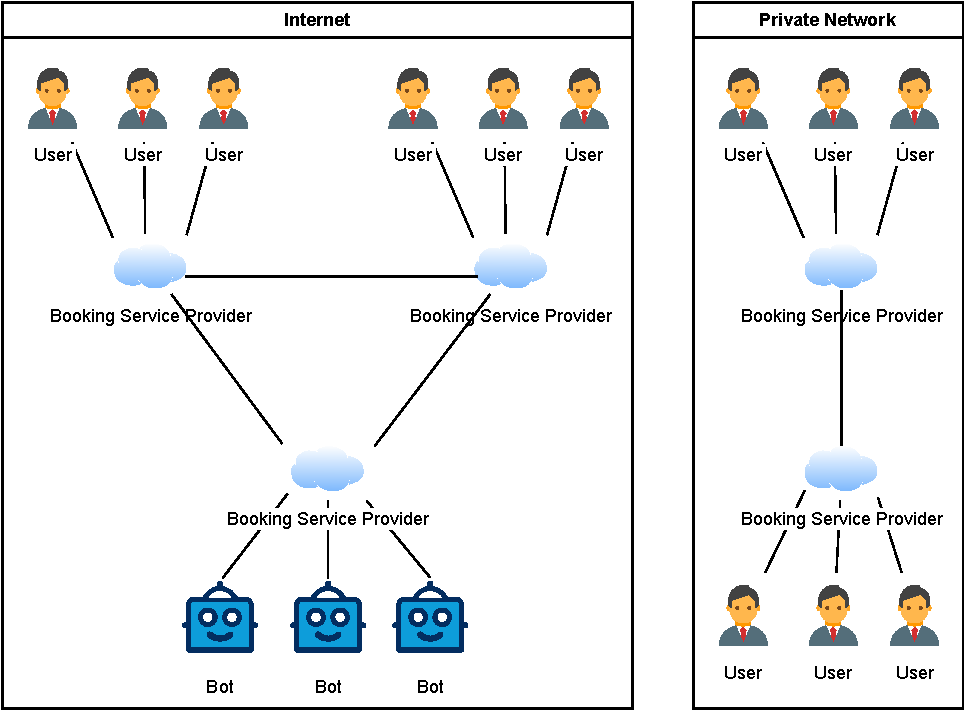
\includegraphics[width=1.0\textwidth]{content/design/system_network_diagram.drawio.pdf}
    \caption[System network diagram]{System network diagram}
    \label{fig:system_network_diagram}
\end{figure}

\begin{figure}
    \centering
    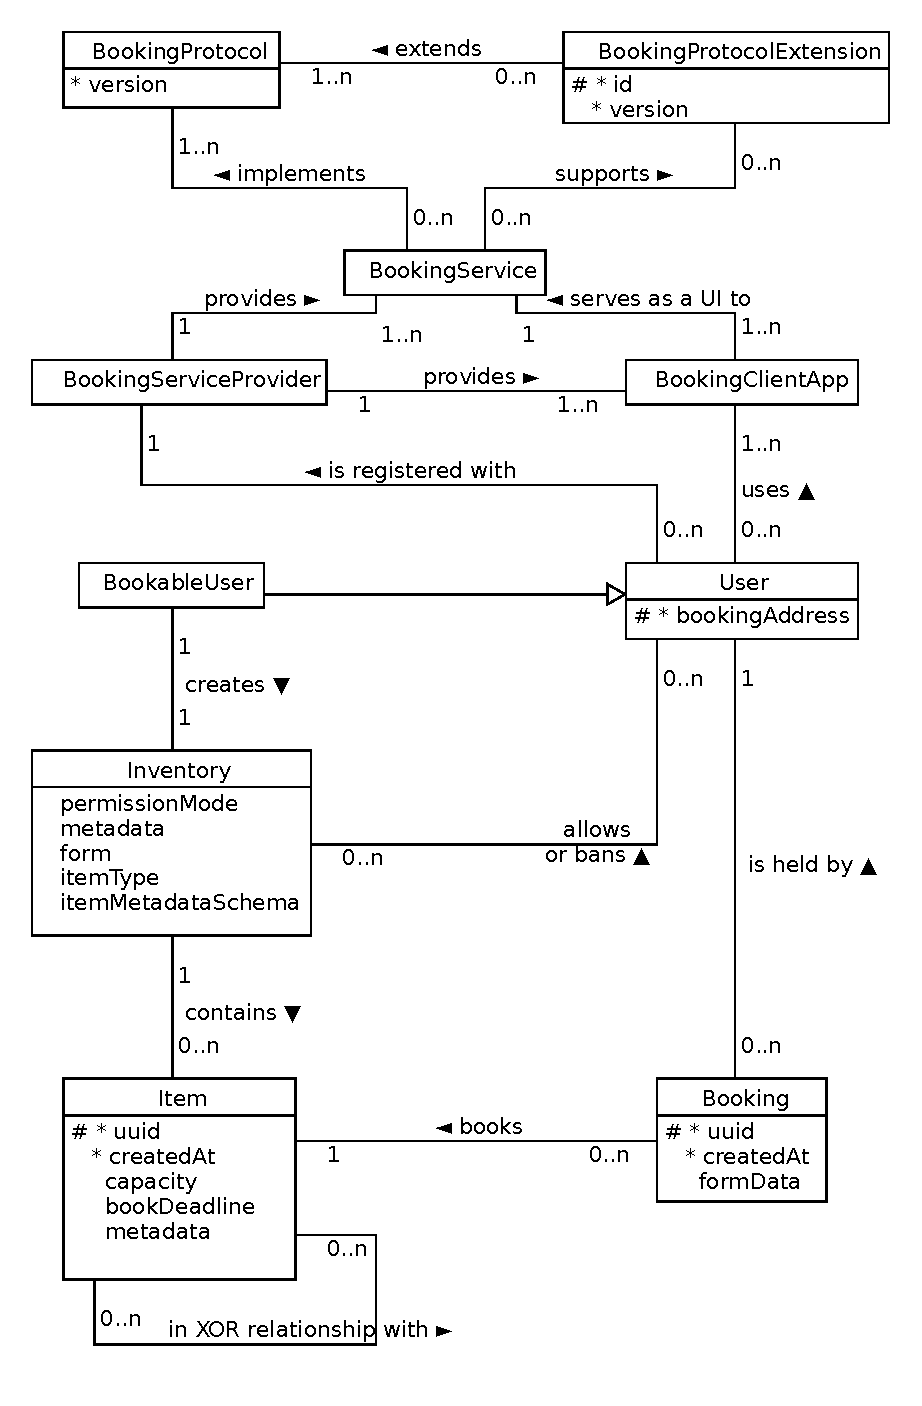
\includegraphics[width=1.0\textwidth]{content/design/system_conceptual_schema.uxf.svg.pdf}
    \caption[System conceptual schema]{System conceptual schema}
    \label{fig:system_conceptual_schema}
\end{figure}

\subsection{Booking address format}

To uniquely identify users in the system, a booking address shall be used. The booking address is a string that is unique within the system, and it is registered with the user's booking service provider (that being anyone who is an owner of a domain name and runs infrastructure implementing the booking protocol). This is a very familiar idea to that of email addresses and the format will look very similar.

The booking address shall comprise of a username and either a domain name or an Internet Protocol (IP) address, separated by the \textit{at} (\mintinline{text}{@}) sign. At the end of the string, a port may also be specified, separated by a colon. The default port for the booking protocol shall be \mintinline{text}{3080}, and it is not necessary to specify it in the booking address if it is the default.

The port \mintinline{text}{3080} is, according to~\cite{neo4j_ports}, not restricted in browsers and, according to~\cite{rfc6335} is in the range of \enquote{User Ports} which range from \mintinline{text}{1024} to \mintinline{text}{49151}, as opposed to \enquote{System Ports} which are below this range, and \enquote{Dynamic Ports} which are above the range and are never assigned by the Internet Assigned Numbers Authority (IANA). Searching for the port usage using search engines and using IANA's Service Name and Transport Protocol Port Number Registry~\cite{iana_ports} has not shown too widespread use of the port number.

\begin{sloppypar}
The booking address shall be case-insensitive, to prevent user errors. The username part may contain the 26 (case-insensitive) Latin letters, Arabic numerals, and the following special characters: the period (\mintinline{text}{.}), the hyphen/minus character (\mintinline{text}{-}), and an underscore (\mintinline{text}{_}). The username can be expressed by the regular expression \mintinline{text}{[0-9A-Za-z._-]+}. The entire booking address can then be expressed as \mintinline{text}{<username>@<ip_address>[:port]} and \mintinline{text}{<username>@<domain_name>[:port]}. Example valid booking addresses include \mintinline{text}{alice@127.0.0.1}, \mintinline{text}{bob@localhost:3080}, and \mintinline{text}{john.doe98@example.com}. Example booking addresses that are considered equivalent are \mintinline{text}{john.doe98@example.com}, \mintinline{text}{john.doe98@example.com:3080}, and \mintinline{text}{John.Doe98@example.com}. The maximum length of the username part shall be 64 characters (similarly to the limit of the local part of an email address, as defined by~\cite{rfc5321}).
\end{sloppypar}

\subsection{Custom URL scheme}

According to~\cite{google_pwa_uri}: \enquote{A Uniform Resource Identifier (URI) is a compact sequence of characters that identifies an abstract or physical resource. Each URI begins with a scheme name that refers to a specification for assigning identifiers within that scheme. As such, the URI syntax is a federated and extensible naming system wherein each scheme's specification may further restrict the syntax and semantics of identifiers using that scheme. Schemes are also known as protocols.} Not to be confused with the actual communication protocol. URLs are a subset of URIs that specifies the location of a resource on the internet.

In order to differentiate booking addresses from other identifiers when shared around the Web and enable users to assign their booking client application of choice to handle activated booking address hyperlinks, a custom URL scheme is also designed. \cite{google_pwa_uri}~states that in order for a progressive web application (PWA) to register their ability to open or handle particular URL schemes, the scheme must either be one of a few safelisted schemes or be prefixed with \mintinline{text}{web+}. Of course, this does not restrict non-PWA applications from handling the scheme.

\begin{sloppypar}
In order to future-proof the system and alow the increasingly popular PWAs to handle the scheme, the booking system shall use the scheme \mintinline{text}{web+booking}. Searches made using search engines for the exact phrase have not revealed any existing use of the scheme. The scheme shall be followed by a booking address and, optionally, any of the following (in the order listed):~a path separated from the booking address by a forward slash (\mintinline{text}{/}), query parameters separated from prior URI segments by a question mark (\mintinline{text}{?}), separated from each other by an ampersand (\mintinline{text}{&}) and separated from their own values by an equals sign (\mintinline{text}{=}), and lastly a fragment separated from prior URI segments by a number sign (\mintinline{text}{#}), much like in the case of URLs.
\end{sloppypar}

The path, query, and fragment segments will not be utilized in the initial version of the booking protocol, but extensions of the protocol as well as newer protocol versions may utilize them in the future. As an example of possible future utilization of these segments, path and fragment could be used to direct the client application to a certain section and the parameters could be used to provide additional functionality, such as form filling with predefined values or item filtering and sorting.

Because of limitations of URL format, unlike in URIs, the \textit{at} (\mintinline{text}{@}) sign in cannot be used in the booking booking address in the URL, and using a percent encoding would mean double encoding. Therefore, specifically in booking schema URLs, it shall be replaced with the \textit{tilde} (\mintinline{text}{~}) character, which can be used and easily separated from the rest of the URL.

\begin{sloppypar}
The URL scheme can then be expressed as \mintinline{text}{web+booking://<booking_address>[/path][?query][#fragment]}. Example URIs include the following:
\begin{itemize}
    \item \mintinline{text}{web+booking://alice~127.0.0.1},
    \item \mintinline{text}{web+booking://bob~localhost/a},
    \item \mintinline{text}{web+booking://charlie~localhost:3080?q=val},
    \item \mintinline{text}{web+booking://dan~localhost:8000#section},
    \item and \mintinline{text}{web+booking://john.doe98~example.com/a?b=1&c=2&d=3#e}.
\end{itemize}
\end{sloppypar}

\subsection{Implementation architecture}

The implementation will use the microservice architecture API gateway pattern, with each service being containerized. A diagram illustrating the architecture is shown in the figure~\ref{fig:architecture_diagram}. The figure~\ref{fig:architecture_diagram_detailed} then shows a more detailed diagram of the architecture featuring the technologies chosen for each service (which are later described in the section~\ref{part:implementation}).

This will enable more efficient scaling of the individual services, as well as easier replacement of one individual service, if for instance a booking service provider decides to use their own implementation of only one of the services. It is also in accordance with the non-functional requirement~\ref{req:cloud_native}.

\begin{figure}
    \centering
    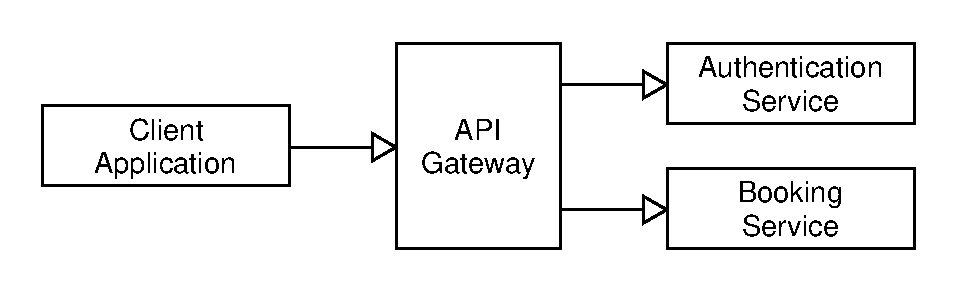
\includegraphics[width=1.0\textwidth]{content/design/architecture_diagram.pdf}
    \caption[Architecture diagram]{Architecture diagram}
    \label{fig:architecture_diagram}
\end{figure}

\begin{figure}
    \centering
    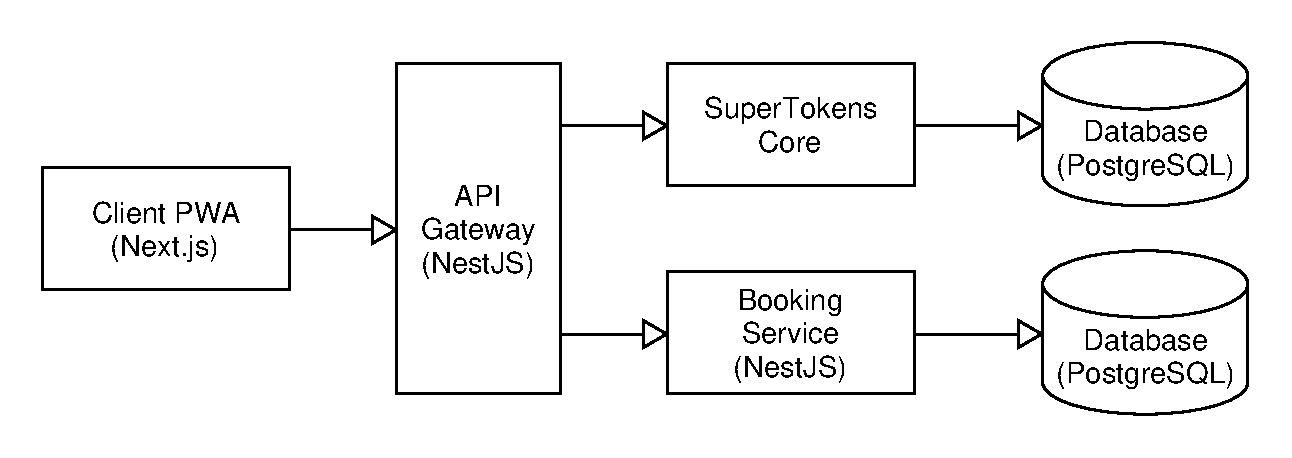
\includegraphics[width=1.0\textwidth]{content/design/architecture_diagram_detailed.pdf}
    \caption[Detailed architecture diagram]{Detailed architecture diagram}
    \label{fig:architecture_diagram_detailed}
\end{figure}


\section{Booking Protocol}
\label{part:booking_protocol}

The booking protocol shall build upon the HTTP protocol. Because the booking protocol shall handle transfers of lots of personal data, outside of localhost the secured HTTP variant HTTPS shall be used (which is also enforced by some web browsers). The booking protocol shall use JSON as the data format for all requests and responses. In the headers of every request and response, two header items shall be present: \texttt{Booking-address} and \texttt{Booking-Service-Info}.

The \texttt{Booking-Address} header shall contain the booking address of the user who (or on whose behalf was) made the request. The receiving booking service shall then verify, that the request is coming from a server, whose IP address belongs to the domain of the booking address (if it uses a domain and not an IP address) according to public DNS records. This can be done using reverse DNS queries. If the booking service is unable to verify the booking address, it shall throw an HTTP 401 error with an informative message.

The \texttt{Booking-Service-Info} header shall contain base64 encoded JSON string, which contains information about the booking service, namely its supported protocol version and protocol extensions (and their versions). The receiving booking service shall throw an HTTP 400 error with an informative message, if it is not compatible with the requesting booking service (or if the request is missing the header). The decoded and parsed object can be described by a TypeScript interface as shown in the listing~\ref{code:booking_protocol_service_info_interface}.

\begin{listing}
    \inputminted[breaklines]{typescript}{content/design/booking_protocol_service_info_interface.ts}
    \caption{Definition of booking service info JSON using a TypeScript interface}
    \label{code:booking_protocol_service_info_interface}
\end{listing}

Furthermore, each request (not response) shall contain the \texttt{Host} header, with the host of the target booking service, so that the booking service, which can be hosted on multiple domains under one IP address, can determine the target booking address.

The booking protocol shall use the following two endpoints:
\begin{itemize}
    \item \texttt{GET /users/:username} -- Get a bookable user's inventory with items.
    \begin{itemize}
        \item The path parameter \texttt{:username} shall contain username part of the booking address of the user whose inventory is requested.
        \item Respond with HTTP 200 and the \texttt{Inventory} resource with its items included and item occupancy (number of bookings of the item) calculated. The resource can be described by a TypeScript interface as shown in the listing~\ref{code:booking_protocol_inventory_interface}.
        \item Respond with HTTP 404 if the booking address requested by the combination of the username from the path and host from the Host header does not exist.
    \end{itemize}
    \item \texttt{POST /users/:username/bookings} -- Create a booking for an item from a bookable user's inventory.
    \begin{itemize}
        \item The path parameter \texttt{:username} shall contain username part of the booking address of the user whose item is being booked.
        \item The request body shall contain the \texttt{Booking} resource with the booked item's id. The resource can be described by a TypeScript interface as shown in the listing~\ref{code:booking_protocol_booking_interface}.
        \item Respond with HTTP 201 and the \texttt{BookingWithItem} resource with its item included and item occupancy (number of bookings of the item) calculated. The resource can be described by a TypeScript interface as shown in the listing~\ref{code:booking_protocol_booking_with_item_interface}.
        \item Respond with HTTP 400 if the booking is after book deadline, fully booked, or the given form data does not match the JSON schema in the item.
        \item Respond with HTTP 404 if the booking address requested by the combination of the username from the path and host from the Host header does not exist, or if the item requested for booking does not exist.
        \item Respond with HTTP 409 if the booking already exists.
        \item Note that it is up to the requesting user's booking service to store the booking (and item or inventory) data if it wants to enable its users to view their bookings and items later.
    \end{itemize}
\end{itemize}

\begin{listing}
    \inputminted[breaklines]{typescript}{content/design/booking_protocol_inventory_interface.ts}
    \caption{Definition of \texttt{Inventory} resource JSON using a TypeScript interface}
    \label{code:booking_protocol_inventory_interface}
\end{listing}

\begin{listing}
    \inputminted[breaklines]{typescript}{content/design/booking_protocol_booking_interface.ts}
    \caption{Definition of \texttt{Booking} resource JSON using a TypeScript interface}
    \label{code:booking_protocol_booking_interface}
\end{listing}

\begin{listing}
    \inputminted[breaklines]{typescript}{content/design/booking_protocol_booking_with_item_interface.ts}
    \caption{Definition of \texttt{BookingWithItem} resource JSON using a TypeScript interface}
    \label{code:booking_protocol_booking_with_item_interface}
\end{listing}

\subsection{Use case}

The booking protocol will be used for a simple use case of a business that occasionally holds one-time events and it wants to know names, emails, and optionally phones of the users who are interested in attending. The business will use the booking protocol to allow users to book a spot at the event. The business will have a booking service, which will be used by the users to book a spot at the event.

The business also wants to let the users know its name, description, website, and contact information including email, phone, physical location, and opening hours. Each event (item of the inventory) will have a deadline for booking, a maximum number of bookings, duration, physical location, website, and a form schema, which the users must fill in when booking a spot at the event. The form schema will be a JSON schema, which will be used to validate the form data sent by the users when booking a spot at the event.


\section{Booking Service}
\label{part:booking_service}

The booking service shall implement the booking protocol designed in \ref{part:booking_protocol}. Furthermore, it shall offer internal APIs for use by the booking client application.

\subsection{Database}
\label{part:booking_service_database}

This section describes the design decisions behind the structure of the database and the choice of the database engine.

\subsubsection{Conceptual Schema}
\label{part:conceptual_schema}

The data that will need to be stored in the database can be described by the conceptual schema in figure~\ref{fig:db_conceptual_schema}. The database will need to store information about users, inventories, items, bookings, and the relationships between them. Most of the data is highly relational, with some properties being JSON documents. Either one database with support for both relational and document data types, or two separate databases, one for relational data and one for document data, could be used.

\begin{figure}
    \centering
    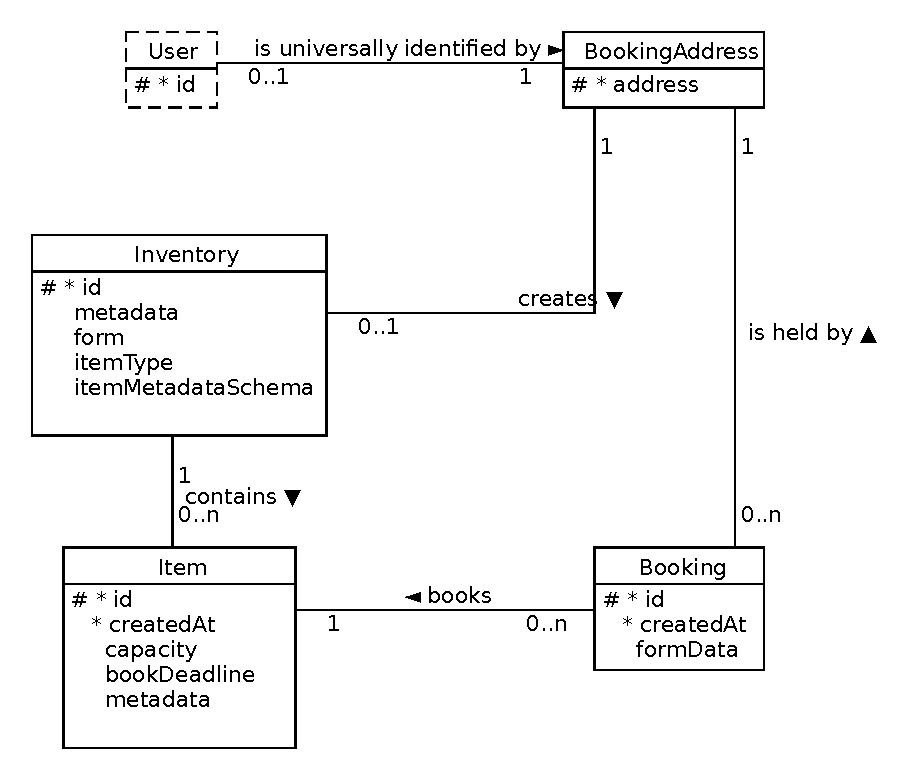
\includegraphics[width=1.0\textwidth]{content/design/db_conceptual_schema.uxf.svg.pdf}
    \caption[Conceptual schema of the booking service database]{Conceptual schema of the booking service database}
    \label{fig:db_conceptual_schema}
\end{figure}

\subsubsection{OLAP vs. OLTP}
\label{part:olap_vs_oltp}

When determining which database engine to use and how to structure the database, one aspect to examine is whether the system will be used for online analytical processing (OLAP) or online transaction processing (OLTP). This system is a prime example of OLAP

\subsubsection{ACID vs. BASE}
\label{part:acid_vs_base}

According to~\cite{brewer_cap, ibm_cap}, consistency, availability, and partition tolerance are the three properties that are impossible to achieve simultaneously in a distributed system. This is known as the CAP theorem. In the context of databases, the CAP theorem is often discussed in terms of ACID (Atomicity, Consistency, Isolation, Durability) and BASE (Basically Available, Soft state, Eventually consistent) properties.

In the domain of booking, strong consistency and availability is absolutely essential. For example, an item available for booking must never be booked by more users than its capacity. Bookings are can also be very time sensitive. For those reasons, the system must be designed with ACID properties in mind.


\section{Client Application}
\label{part:client_application}

The booking client application shall use a single page application (SPA) architecture. The SPA architecture is a design pattern that allows the client application to load a single HTML page and dynamically update the page as the user interacts with the application. This design pattern allows the client application to be more responsive and provide a better user experience.

The client application will be a progressive web application (PWA) that can be installed on the user's device and possibly even work offline (though that will not be implemented as of now). This will also enable the use of the custom booking URL schema (on supported platforms). And as any web application, it will be accessible on many different devices and platforms.

Lastly, it will be a mobile-first design to ensure that the application is usable on mobile devices.

Initially, the Figma design tool was used to create wireframes of the UI, however, the UI has changed by a not significant amount since then, so the original design is left out of the thesis.



% ----------------------------------------- Implementation -----------------------------------------

\chapter{Implementation}
\label{part:implementation}

This chapter describes the prototype implementation of the designed system, as well as its testing and evaluation.

For the entire implementation, TypeScript, Node.js, and npm were used. The reason behind this choice is both prior experience with this ecosystem of the author of this thesis, as well as its popularity for full-stack web development, ensuring high amount of useful supporting resources.

TypeScript~\cite{typescript} is a popular \enquote{strongly typed programming language that builds on JavaScript.} It \enquote{adds additional syntax to JavaScript to support a tighter integration with (...) an editor} to \enquote{catch errors early.} The code \enquote{converts to JavaScript, which runs anywhere JavaScript runs: in a browser, on Node.js, Deno, Bun.} TypeScript is a static type checker, meaning that it performs type checking only at compile time, not during the runtime.

\begin{sloppypar}
Node.js~\cite{node_js} is a \enquote{cross-platform JavaScript runtime environment that lets developers create servers, web apps, command line tools and scripts.} It is \enquote{built on the V8 JavaScript engine} (which is also used~\cite{v8} by Chromium-based web browsers, such as Google Chrome). The Node.js documentation~\cite{node_js} further states that \enquote{npm is the standard package manager for Node.js,} with npm~\cite{npm} claiming that it is \enquote{the largest software registry in the world.}
\end{sloppypar}

Each application that is part of the implementation is kept in a separate directory: \textit{booking-service} for the booking service, \textit{booking-api-gateway} for the API gateway, and \textit{booking-client-app} for the client application. These directories with the source code are included in the content of the digital attachment~\ref{part:contents_of_the_digital_attachment}.

\begin{sloppypar}
Every application directory contains a \textit{package.json} file and an \textit{npm-shrinkwrap.json} file. These files in the JavaScript Object Notation (JSON) data format are both related to npm, with \textit{package.json}~\cite{npm_docs} describing many things, including general metadata about the project (package name, version adhering to semantic versioning, license information, author information, important URLs, etc.), npm scripts' definitions, lists of npm dependencies (of various types) along with their version, application entrypoints, and information about supported environments. The file \textit{npm-shrinkwrap.json} is then generated by npm when installing dependencies (using the \mintinline{sh}{npm install} command) and it is a publishable variant of the \textit{package-lock.json} file used by default to describe \enquote{the exact (dependency) tree that was generated, such that subsequent installs are able to generate identical trees, regardless of intermediate dependency updates.} This ensures consistently reproducible dependency installations. Dependencies are installed into the \textit{node\_modules} directory of each project (this directory is not included in the source code).
\end{sloppypar}

To fulfill non-functional requirement~\ref{req:open_source}, each application directory also contains a \textit{LICENSE.txt} file with the popular permissive open-source MIT license (which is also correctly denoted in the \textit{package.json} files) and each application only uses dependencies with compatible permissive open-source licenses.

Furthermore, the file \textit{Containerfile} is included in each application directory. \textit{Containerfile}~\cite{podman_github} (which is an alternative name for \textit{Dockerfile}) is \enquote{a configuration file that automates the steps of creating a container image.} Application container images can then be created using tools like Docker, Podman, and Buildah, either in the Docker image format or in the Open Container Initiative (OCI) image format (which is largely similar). These container images can then used by orchestration tools (such as Kubernetes) for~\cite{kubernetes} \enquote{automating deployment, scaling, and management of (...) applications}. Additionally, the \textit{compose.prod.yaml} Compose file is attached to enable easily building and running all the service containers in production mode using tools like Docker Compose, and the \textit{booking-service} directory contains a \textit{compose.yaml} file with the dependant services for the booking service to run (and thus is useful for development). This fulfills non-functional requirement~\ref{req:cloud_native}.

Lastly, each application directory contains a \textit{README.md} file in the Markdown format, describing how to run it, and a \textit{.env.template} file with a template for the environment variables that need to be set for the application to run.

\section{Booking Service}
\label{part:i_booking_service}

The booking service shall implement the booking protocol designed in \ref{part:booking_protocol}. Furthermore, it shall offer internal APIs for use by the booking client application.

\subsection{Database}
\label{part:booking_service_database}

This section describes the design decisions behind the structure of the database and the choice of the database engine.

\subsubsection{Conceptual Schema}
\label{part:conceptual_schema}

The data that will need to be stored in the database can be described by the conceptual schema in figure~\ref{fig:db_conceptual_schema}. The database will need to store information about users, inventories, items, bookings, and the relationships between them. Most of the data is highly relational, with some properties being JSON documents. Either one database with support for both relational and document data types, or two separate databases, one for relational data and one for document data, could be used.

\begin{figure}
    \centering
    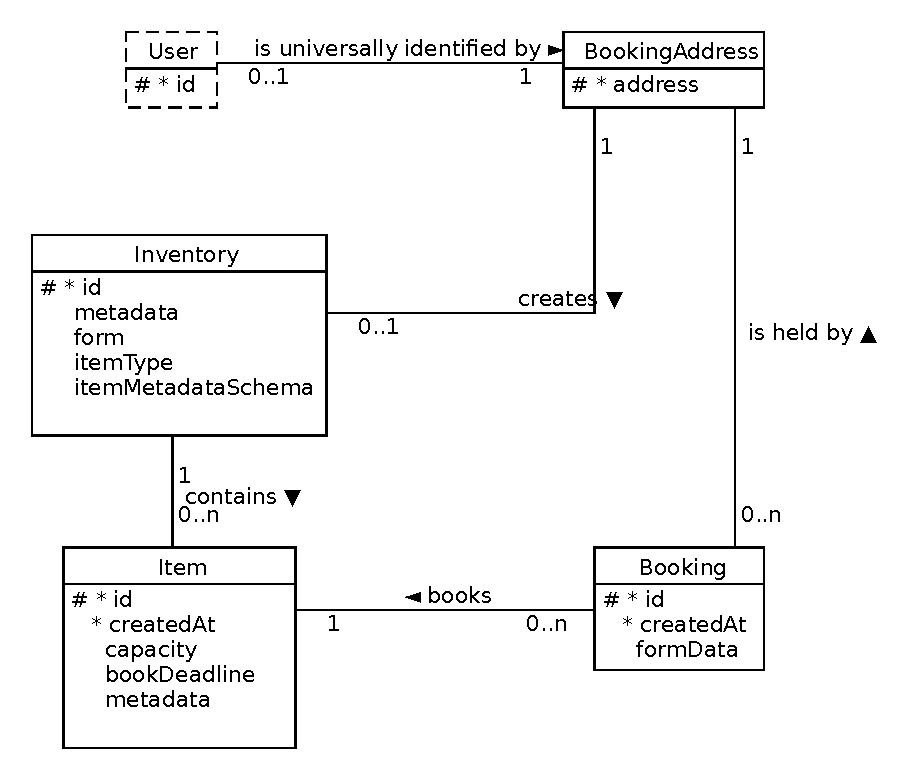
\includegraphics[width=1.0\textwidth]{content/design/db_conceptual_schema.uxf.svg.pdf}
    \caption[Conceptual schema of the booking service database]{Conceptual schema of the booking service database}
    \label{fig:db_conceptual_schema}
\end{figure}

\subsubsection{OLAP vs. OLTP}
\label{part:olap_vs_oltp}

When determining which database engine to use and how to structure the database, one aspect to examine is whether the system will be used for online analytical processing (OLAP) or online transaction processing (OLTP). This system is a prime example of OLAP

\subsubsection{ACID vs. BASE}
\label{part:acid_vs_base}

According to~\cite{brewer_cap, ibm_cap}, consistency, availability, and partition tolerance are the three properties that are impossible to achieve simultaneously in a distributed system. This is known as the CAP theorem. In the context of databases, the CAP theorem is often discussed in terms of ACID (Atomicity, Consistency, Isolation, Durability) and BASE (Basically Available, Soft state, Eventually consistent) properties.

In the domain of booking, strong consistency and availability is absolutely essential. For example, an item available for booking must never be booked by more users than its capacity. Bookings are can also be very time sensitive. For those reasons, the system must be designed with ACID properties in mind.


\section{API Gateway}
\label{part:i_api_gateway}

The API gateway behaves to the outside worlds as a booking service. It lets anybody access the booking protocol APIs of the booking service, but only authenticated users to use to internal APIs meant for the booking client app.

Much like the booking service, the API gateway was built around the framework NestJS (Nest), with Express enabled.

For user authentication, the library SuperTokens was used. For proxying requests to booking service, the library http-proxy-middleware was used.

The API gateway also provides on internal endpoint \texttt{POST /forward-booking-request} for use by the booking service only, which is used to forward booking requests from the booking service to remote booking services.


\section{Client Application}
\label{part:i_client_application}

The booking client application shall use a single page application (SPA) architecture. The SPA architecture is a design pattern that allows the client application to load a single HTML page and dynamically update the page as the user interacts with the application. This design pattern allows the client application to be more responsive and provide a better user experience.

The client application will be a progressive web application (PWA) that can be installed on the user's device and possibly even work offline (though that will not be implemented as of now). This will also enable the use of the custom booking URL schema (on supported platforms). And as any web application, it will be accessible on many different devices and platforms.

Lastly, it will be a mobile-first design to ensure that the application is usable on mobile devices.

Initially, the Figma design tool was used to create wireframes of the UI, however, the UI has changed by a not significant amount since then, so the original design is left out of the thesis.


\section{Testing and Evaluation}
\label{part:testing_and_evaluation}

First, every part of the implementation was tested manually by the author of this thesis. For the client application, this meant clicking through every page and state, testing edge-case inputs (invalid usernames, booking addresses, form data) and even setting up booking service failure scenarios by temporarily modifying the booking service to respond with invalid data. For the API gateway and the booking service, the command line utility cURL was used to send both valid and invalid requests, including different HTTP header combinations.

Afterwards, when the implementation appeared stable, user usability testing was performed. 

\subsection{Usability testing}

Usability testing was performed with three subjects. \textbf{Subject A} is a 26 year old male software engineer with a university degree, who lives in the suburbs of Prague. \textbf{Subject B} is a 31 year old male army soldier, who lives in Prague. \textbf{Subject C} is a 52 year old female business manager, who lives in the suburbs of Prague and is not too technologically savvy.

The following scenario was chosen based on the designed use case and given to testing subjects: \enquote{You are a manager at a mid-sized business (a couple hundred employees). Your company wants to organize a conference and needs to keep track of how many and who can partake. You know that you yourself will be at the conference.}

Then, the following tasks were given to each subject:
\begin{enumerate}
    \item \enquote{Create a new account and booking address.}
    \item \enquote{Create a new inventory with basic information about yourself as a manager.}
    \item \enquote{Create a new inventory item for the conference.}
    \item \enquote{Make a new booking of the conference item, since you know that you will be participating.}
    \item \enquote{Check if you can find your booking in the inventory.}
\end{enumerate}

The testing was done in person, on a Windows 11 laptop that was brought to the testing setting, with all the required services set up and the booking client application open in the latest Google Chrome browser.

The testing subjects performed the tasks as follows:
\begin{enumerate}
    \item Account and address creation:
    \begin{itemize}
        \item \textbf{Subject A} signed in using their GitHub account, input a valid username and the first try and created their booking address.
        \item \textbf{Subject B} took a moment to find out how to switch the sign-in component to the sign up state, then created an account with email and password. They input a username and created their booking address, though at first try they put in an invalid character for the username, which was quickly corrected thanks to the instant UI feedback.
        \item \textbf{Subject C} tried to fill in the email and password for their new account into the sign in form. When that attempt was unsuccessful, they realized the presence of the button to switch the component to the sign up state and created their new account successfully. Then they put in a simple username and created a booking address without an issue.
    \end{itemize}
    \item Inventory creation:
    \begin{itemize}
        \item \textbf{Subject A} immediately spotted the burger icon button that opens the drawer with a link to the business section, where they transitioned, filled out the new inventory form and created their inventory.
        \item \textbf{Subject B} first opened the profile dialog, but their second choice was the burger icon button. The subject created their inventory without issue.
        \item \textbf{Subject C} took a little while to look around the page, but their first choice was the burger icon button. The rest of the process was flawless.
    \end{itemize}
    \item Item creation:
    \begin{itemize}
        \item \textbf{Subject A} navigated to the add item page and filled out the form. They were experimenting with the duration field, which they said has a too exotic format, though it was not needed for this task. Then they proceeded to create the item.
        \item \textbf{Subject B} navigated to the add item page, filled out the form and added the item to the inventory.
        \item \textbf{Subject C} also navigated to the add item page, filled out the form and added the item to the inventory without anything to mention.
    \end{itemize}
    \item Item booking:
    \begin{itemize}
        \item \textbf{Subject A} first clicked the newly created item, then realized that they need to navigate back to the home page and then to the new booking page. They at first did not realize, that they need to input the whole booking address, but thanks to the instant feedback of the UI, they managed to get to the items for booking page and complete the booking.
        \item \textbf{Subject B} experienced the same issues as \textbf{Subject A}, but managed to complete the booking.
        \item \textbf{Subject C} also struggled to get to the correct page and then to find out what to input as the booking address. Once they got over this step, the process was straightforward.
    \end{itemize}
    \item Booking overview:
    \begin{itemize}
        \item \textbf{Subject A} finished the task successfully without anything to mention.
        \item \textbf{Subject B} accessed the booking through their home page and thought that they completed the task. They had to be told, that this is not the correct place, otherwise they would not complete the task successfully.
        \item \textbf{Subject C} first opened the booking through their home page, then re-read the instructions and went correctly to their inventory to access the booking.
    \end{itemize}
\end{enumerate}

\subsection{Evaluation}

Through the conducted usability testing, some UI/UX blind spots were found. The issues some users faced with the sign in form could be attributed to the fact, that the form was in English and neither were native English speakers, so the two similar terms \enquote{sign in} and \enquote{sign up} can be confusing. Improvements in the client application could be made to better parse user values of certain metadata (enabling for example more human readable duration or opening hours format). Some sections of the client app are very similar, which can be also confusing. Likely the biggest hurdle is the exotic nature of booking addresses. This issue could be improved by displaying the users' booking addresses more prominently in the application.

These issues, however, are relatively minor and the implementation is fully functional and fulfills the designed use case.



% ------------------------------------------- Conclusion -------------------------------------------

\begin{conclusion}
	\label{part:conclusion}
	The goal of this thesis was to design an open and decentralized, general-purpose online reservation system architecture, including a common HTTP-based client-server protocol, and developing a reference implementation including both a client application and a back end. The created solution was to be easy to integrate with state-of-the-art cloud-native architectures, and was to support a use case for a selected type of reservation business. Possible extensions for the selected use case were to be discussed. The reference implementation was to be tested and evaluated for the selected use case.

First, a research/overview of select existing online reservation systems was conducted in chapter~\ref{part:existing_reservation_systems}. Based on the results of the research, the assignment of the thesis, as well as original ideas, a requirements analysis was made in chapter~\ref{part:analysis}, including both functional and non-functional requirements for the system to be designed and implemented. Chapter~\ref{part:design} describes the design of the newly created system, including its architecture, the common protocol, a use case for the system, the back-end services, and the client application. Finally, chapter~\ref{part:implementation} describes the implementation of the system based on the created design, as well as its testing and evaluation, fulfilling the selected use case.

The research on the existing online reservation systems could additionally be useful to those who are in the near future looking for a reservation system. Furthermore, together with the requirements analysis, this information could be useful to those who are looking into developing a reservation system of their own. The approaches in the design and implementation chapters can, in part, be used as a reference for those who are looking into developing other applications with some of the technologies or techniques used here. The designed architecture and protocol can be used by others to create new interoperable implementations. And, lastly, the implemented prototype can be further developed into a production-ready system, or integrated into existing infrastructures, as it is released under a permissive open-source license.

One can dream of a future where, if the ideas proposed in this thesis ever became a commonplace reality, after searching for a hairdresser nearby using a search engine, users would be presented with a list of results including not only the basic information about hair salons within close proximity, but also with real-time information about the hairdressers' availability (based on which the results could also be sorted), and a direct link to book an appointment, which would open a user's booking client application of choice, that would in turn automatically fill out the user's personal data if required by the business offering the appointment, and let the user just confirm the booking. Or a future where users could have their booking service automatically book an appointment with their dentist for regular check-ups twice a year, with the exact time and date chosen based on the availability of both parties and an optional notification about the newly created booking.

\end{conclusion}

% ------------------------------------------ Bibliography ------------------------------------------

\begin{sloppypar}
	\printbibliography
\end{sloppypar}

% --------------------------------------- Appendix chapters ----------------------------------------

\appendix

% ---------------------------------------- List of Acronyms ----------------------------------------

\chapter{List of Acronyms}
\label{part:list_of_acronyms}

\begin{description}
	\item[ACID] Atomicity, consistency, isolation, durability
	\item[AI] Artificial intelligence
	\item[API] Application programming interface
	\item[BASE] Basically available, soft state, eventually consistent
	\item[CAP] Consistency, availability, partition tolerance
	\item[CLI] Command-line interface
	\item[CSS] Cascading Style Sheets
	\item[CSV] Comma-separated values
	\item[GUI] Graphical user interface
	\item[HTTP] Hypertext Transfer Protocol
	\item[IP] Internet Protocol
	\item[IANA] Internet Assigned Numbers Authority
	\item[IRI] Internationalized Resource Identifier
	\item[JSON] JavaScript Object Notation
	\item[JSON-LD] JavaScript Object Notation for Linked Data
	\item[OCI] Open Container Initiative
	\item[OLAP] Online analytical processing
	\item[OLTP] Online transaction processing
	\item[ORM] Object relational mapping
	\item[PWA] Progressive web application
	\item[SDK] Software development kit
	\item[SEO] Search engine optimization
	\item[UI] User interface
	\item[URI] Uniform Resource Identifier
	\item[URL] Uniform Resource Locator
	\item[UUID] Universal Unique Identifier
	\item[UX] User experience
\end{description}


% ------------------------------- Contents of the Digital Attachment -------------------------------

\chapter{Contents of the Digital Attachment}
\label{part:contents_of_the_digital_attachment}

\begin{figure}
	\dirtree{%
		.1 implementation\DTcomment{the source code of the implementation}.
			.2 booking-api-gateway\DTcomment{booking API gateway}.
			.2 booking-client-app\DTcomment{booking client application}.
			.2 booking-service\DTcomment{booking service}.
			.2 compose.prod.yaml\DTcomment{a production-mode Compose file}.
			.2 README.md\DTcomment{Markdown instructions to the implementation source code}.
		.1 thesis.
			.2 MT\_Straka\_David\_2025.pdf\DTcomment{thesis text PDF}.
			.2 MT\_Straka\_David\_2025\DTcomment{\LaTeX{} source of the thesis text}.
	}
\end{figure}


% -------------------------------------- End of the document ---------------------------------------

\end{document}
